%%% Hlavní soubor. Zde se definují základní parametry a odkazuje se na ostatní části. %%%

%% Verze pro jednostranný tisk:
% Okraje: levý 40mm, pravý 25mm, horní a dolní 25mm
% (ale pozor, LaTeX si sám přidává 1in)
\documentclass[12pt,a4paper]{report}
\setlength\textwidth{145mm}
\setlength\textheight{247mm}
\setlength\oddsidemargin{15mm}
\setlength\evensidemargin{15mm}
\setlength\topmargin{0mm}
\setlength\headsep{0mm}
\setlength\headheight{0mm}
% \openright zařídí, aby následující text začínal na pravé straně knihy
\let\openright=\clearpage

%% Pokud tiskneme oboustranně:
% \documentclass[12pt,a4paper,twoside,openright]{report}
% \setlength\textwidth{145mm}
% \setlength\textheight{247mm}
% \setlength\oddsidemargin{14.2mm}
% \setlength\evensidemargin{0mm}
% \setlength\topmargin{0mm}
% \setlength\headsep{0mm}
% \setlength\headheight{0mm}
% \let\openright=\cleardoublepage

%% Vytváříme PDF/A-2u
\usepackage[a-2u]{pdfx}

%% Přepneme na českou sazbu a fonty Latin Modern
\usepackage[slovak]{babel}
\usepackage{lmodern}
\usepackage[T1]{fontenc}
\usepackage{textcomp}

%% Použité kódování znaků: obvykle latin2, cp1250 nebo utf8:
\usepackage[utf8]{inputenc}

%%% Další užitečné balíčky (jsou součástí běžných distribucí LaTeXu)
\usepackage{amsmath}        % rozšíření pro sazbu matematiky
\usepackage{amsfonts}       % matematické fonty
\usepackage{amsthm}         % sazba vět, definic apod.
\usepackage{bbding}         % balíček s nejrůznějšími symboly
			    % (čtverečky, hvězdičky, tužtičky, nůžtičky, ...)
\usepackage{bm}             % tučné symboly (příkaz \bm)
\usepackage{graphicx}       % vkládání obrázků
\usepackage{fancyvrb}       % vylepšené prostředí pro strojové písmo
\usepackage{indentfirst}    % zavede odsazení 1. odstavce kapitoly
\usepackage{natbib}         % zajištuje možnost odkazovat na literaturu
			    % stylem AUTOR (ROK), resp. AUTOR [ČÍSLO]
\usepackage[nottoc]{tocbibind} % zajistí přidání seznamu literatury,
                            % obrázků a tabulek do obsahu
\usepackage{icomma}         % inteligetní čárka v matematickém módu
\usepackage{dcolumn}        % lepší zarovnání sloupců v tabulkách
\usepackage{booktabs}       % lepší vodorovné linky v tabulkách
\usepackage{paralist}       % lepší enumerate a itemize
\usepackage{xcolor}         % barevná sazba

%%% Vlastné balíčky
\usepackage{float}          % pre vkladanie obrázkov

%%% Údaje o práci

% Název práce v jazyce práce (přesně podle zadání)
\def\NazevPrace{ServIS – webový systém pro~firmy zabývající se opravami bagrů}

% Název práce v angličtině
\def\NazevPraceEN{ServIS – a~web system for~companies dealing with~excavator repairs}

% Jméno autora
\def\AutorPrace{Milan Truchan}

% Rok odevzdání
\def\RokOdevzdani{2023}

% Název katedry nebo ústavu, kde byla práce oficiálně zadána
% (dle Organizační struktury MFF UK, případně plný název pracoviště mimo MFF)
\def\Katedra{Katedra distribuovaných a~spolehlivých systémů}
\def\KatedraEN{Department of~Distributed and~Dependable Systems}

% Jedná se o katedru (department) nebo o ústav (institute)?
\def\TypPracoviste{Katedra}
\def\TypPracovisteEN{Department}

% Vedoucí práce: Jméno a příjmení s~tituly
\def\Vedouci{Mgr. Pavel Ježek, Ph.D.}

% Pracoviště vedoucího (opět dle Organizační struktury MFF)
\def\KatedraVedouciho{Katedra distribuovaných a~spolehlivých systémů}
\def\KatedraVedoucihoEN{Department of~Distributed and~Dependable Systems}

% Studijní program a obor
\def\StudijniProgram{Informatika}
\def\StudijniObor{Programování a~vývoj software}

% Nepovinné poděkování (vedoucímu práce, konzultantovi, tomu, kdo
% zapůjčil software, literaturu apod.)
\def\Podekovani{%
Rád by som sa poďakoval vedúcemu práce~Mgr.~Pavlovi Ježkovi,~Ph.D. za~jeho vedenie, rady, čas a~trpezlivosť, ktorú mi venoval. Taktiež by som sa chcel poďakovať svojej~rodine, ktorá ma motivovala a~podporovala počas vypracovania tejto práce, ale aj počas~celej doby štúdia.
}

% Abstrakt (doporučený rozsah cca 80-200 slov; nejedná se o zadání práce)
\def\Abstrakt{%
Cieľom tejto práce bolo vytvoriť softvérové dielo pre~malé firmy zaoberajúce sa zemnými a~výkopovými prácami, opravou a~predajom bagrov, ktoré nemajú prístup k~vhodnému softvérovému riešeniu pre~svoju činnosť.

Potreba a~správanie funkcionalít bola prekonzultovaná s~majiteľom jednej z~týchto firiem.

Vzniknutý softvér predstavuje riešenie problému, je schopný zobraziť ponuku~(stroje, prídavné zariadenia) a~umožňuje užívateľom dopyt (v~podobe emailov) na~tieto ponuky. V~aplikácii tiež existuje aukcia, kde sa dražia opravené bagre. Užívatelia si tiež môžu v~aplikácií vytvoriť účet. Vymenované funkcionality môžu využívať prihlásení aj neprihlásení užívatelia. Bežní prihlásení užívatelia nemusia vyplňovať informácie o~sebe vo~formulároch pri~dopytovaní sa na~ponuku. Prihlásení admini majú možnosť spravovať stránku. Tj.~pridávať nové, editovať a~mazať existujúce ponuky, odpovedať na~správy atď.

}
\def\AbstraktEN{%
Abstract.
}

% 3 až 5 klíčových slov (doporučeno), každé uzavřeno ve složených závorkách
\def\KlicovaSlova{%
{Informačný systém} {C\#} {.NET} {Blazor Server} {MySQL}
}
\def\KlicovaSlovaEN{%
{Information system} {C\#} {.NET} {Blazor Server} {MySQL}
}

%% Balíček hyperref, kterým jdou vyrábět klikací odkazy v PDF,
%% ale hlavně ho používáme k uložení metadat do PDF (včetně obsahu).
%% Většinu nastavítek přednastaví balíček pdfx.
\hypersetup{unicode}
\hypersetup{breaklinks=true}

%% Definice různých užitečných maker (viz popis uvnitř souboru)
\include{makra}

%% Titulní strana a různé povinné informační strany
\begin{document}
\include{titulka}

%%% Strana s automaticky generovaným obsahem bakalářské práce

\tableofcontents

%%% Jednotlivé kapitoly práce jsou pro přehlednost uloženy v samostatných souborech
\chapter{Úvod}
\addcontentsline{toc}{chapter}{Úvod}

V~súčasnosti existujú malé firmy, ktoré fungujú ako dodávatelia rôznych drahých produktov. Tieto firmy môžu ponúkať na~predaj okrem nových produktov aj staré produkty, ktoré prešli nejakou opravou. Takisto stojí za~zmienku, že kedže ide o~dodávateľov drahých produktov, tak zákazníci sa najprv s~firmou musia dohodnúť na~detailoch obchodu, a~až potom je možné dodanie produktu.

Spoločným problémom takýchto firiem býva, že ich ľudia nepoznajú. Preto by sa spomínaným firmám hodilo riešenie, ktoré by im umožnilo zviditeľniť ich ponuku produktov. Jednoduché riešenie v~podobe statických stránok v~tomto prípade nestačí, pretože by neumožnilo dynamicky meniť ponuku danej firmy. Použitie nejakého CMS systému~(z~ang. content management system), napr.~Word\-Press, takisto nie je optimálnym riešením, pretože vyžaduje znalosť platformy, ktorá nie je samozrejmesťou.

My sme dostali ponuku na~tvorbu riešenia od~jednej z~takýchto firiem. Konkrétne ide o~firmu, ktorá sa zaoberá predajom a~opravou bagrov (ďalej už len klientská firma). Po~konzultácii s~majiteľom (ďalej už len klient) sme zistili, že klientksá firma ponúka služby v~podobe výkopových prác, predaja a~opravy bagrov, a~takisto predaja prídavných zariadení pre~bagre. Taktiež sme zistili, že doteraz fungovala komunikácia medzi klientskou firmou a~zákazníkmi prostredníctvom telefonátov, emailov alebo sa strany fyzicky stretli a~dohodli obchod. Klient od~nás vyžaduje riešenie, ktoré by spĺňalo požiadavky uvedené v~následujúcej podkapitole.

\section{Požiadavky na systém}

V priebehu niekoľkých stretnutí sme s~klientom prebrali a~vypracovali následujúce požiadavky, ktoré softvér musí spĺňať:

\begin{itemize}
\item \textbf{P1 Roly užívateľa}

Jednou z~požiadaviek je, že softvér má rozlišovať zamestnancov firmy spravujúcich systém (ďalej už len administrátori, resp. administrátor) a~bežných zákazníkov. Obom rolám sa bude zobrazovať len obsah podľa funkcionalít, ktoré majú k~dispozícii. Čiže napr.~zákazník si bude môcť zobraziť detail bagra a~vyjadriť oň nejakým spôsobom záujem, ale nezobrazí sa mu možnosť na~jeho vymazanie. V~prípade administrátora bude možné bager napr.~vymazať, ale nedáva zmysel, aby mohol administrátor vyjadrovať záujem o~bager.

\item \textbf{P2 Predstavenie ponuky zákazníkom}

Ako už bolo spomenuté, klientská firma predáva bagre a~prídavné zariadenia pre~bagre. Klient preto chce, aby bol softvér schopný prezentovať ponuku firmy (bagre a~prídavné zariadenia), pričom hlavná ponuka je tvorená bagrami. Klient vyžaduje, aby po~príchode užívateľa na~domovskú (úvodnú) stránku sa zobrazila hlavná ponuka.

\begin{itemize}
\item \textbf{P2.1 Hlavná ponuka}

Hlavná ponuka predstavuje bagre určitého typu (t.~j.~určitej kombinácie značky a~kategórie). Hlavná ponuka obsahuje opis typu bagrov a~fotku reprezentujúcu daný typ bagrov. Po~rozkliknutí nejakej hlavnej ponuky sa zobrazia bagre typu asociovaného s~vybranou ponukou.

\item \textbf{P2.2 Bager}

Každý bager má obsahovať informácie: názov, značku, kategóriu, opis, fotky a~vlastnosti. Tieto informácie majú byť viditeľné pre~každého užívateľa, t.~j.~ako pre~bežného zákazníka, tak aj pre~administrátora. Navyše má ešte stroj obsahovať informáciu o~náhradných dieloch~-- táto informácia má byť viditeľná iba pre~administrátorov. Navyše môžu existovať bagre, ktoré nepatria do~ponuky a~môžu byť využité výhradne iba v~aukcii (viac o~aukcii v~P4).

\item \textbf{P2.3 Prídavné zariadenie}

Každé prídavné zariadenie má obsahovať informácie: názov, značka, kategória, pre~akú kategóriu strojov je zariadenie určené, opis a~fotky. Tieto informácie majú byť viditeľné rovnako pre~každého užívateľa.

\item \textbf{P2.4 Správa bagrov, prídavných zariadení a hlavných ponúk}

Aby mohol administrátor spravovať bagre, prídavné zariadenia ale takisto aj hlavné ponuky podľa potreby, tak je tiež nutné vytvoriť miesto, ktoré mu ich umožní pridávať, odstraňovať a~editovať.
\end{itemize}

\item \textbf{P3 Posielanie dopytu}

Takisto klient od~softvéru vyžaduje, aby umožnil zákazníkom objednať si daný produkt alebo službu prostredníctvom emailových správ. Bežnou praxou v~tomto odvetví je, že cena strojov sa dopredu neudáva. Zákazník najprv vyjadrí záujem (dopyt), prekonzultujú sa detaily medzi potenciálnym kupcom a~firmou, a~až potom prebehne obchod. Z~tohto dôvodu systém nebude fungovať na~princípe ako bežné internetové obchody (tým sa myslí pridávanie do~košíka s~následnou platbou), ale bude fungovať na~princípe posielania správ~(dopytov).

\begin{itemize}
\item \textbf{P3.1 Dopyt}

Dopyt by mal v~sebe obsahovať informácie o~žiadanom predmete, údaje o~užívateľovi, a~tiež správu užívateľa. Uživateľskými údajmi sa myslí meno, priezvisko, email~-- tie sú povinné údaje. A~takisto telefónne číslo, mesto~-- tie sú nepovinné údaje.
\end{itemize}

\item \textbf{P4 Aukcia}

Keď sme v~predošlých podmienkách spomínali ponuku strojov a~prídavných zariadení, tak išlo o~nové produkty. No ako už bolo skôr spomenuté, klientská firma sa špecializuje aj na~opravu bagrov. Klient vyžaduje, aby mohol administrátor v~systéme vytvoriť aukčnú ponuku, do~ktorej by okrem špecifikovania jej konca a~počiatočnej sumy (vyvolávacej ceny), vedel zaradiť opravený bager, a~aby systém umožnil zákazníkom ponúkať sumy (prvá ponúknutá suma môže byť rovná počiatočnej sume, nasledujúce ponúkané sumy musia mať medzi sebou rozdiel aspoň 100 eur), pričom po~skončení dražby zákazník s~najvyššou ponúknutou sumou vyhráva dražený bager.

\begin{itemize}
\item \textbf{P4.1 Správanie aukcie}

Keď aukcia skončí, systém má upozorniť jej účastníkov (poslať email) na~to, či vyhrali alebo prehrali dražbu. Taktiež má softvér upozorniť administrátora systému na~to, že aukcia skončila a~kto je jej víťazom. V~prípade, že aukcia skončila bez víťaza (nikto sa jej nezúčastnil), tak má softvér dražbu automaticky reštartovať, posunúť termín konca dražby o~týždeň a~upozorniť o~tom administrátora (poslať mu email).

\item \textbf{P4.2 Odpočet a ďalšie údaje}

Okrem toho sa od~nášho softvéru vyžaduje, aby bol pri~každej aukčnej ponuke zobrazený odpočet do~konca danej dražby, počet účastníkov, a~taktiež aktuálna (najvyššia ponúknutá) suma.
\end{itemize}

\item \textbf{P5 Správy}

Keďže posielanie dopytov a~správanie aukcie zahŕňa posielanie emailov administrátorom, tak je tiež žiadúce, aby sa emaily dali prečítať nielen\\z~Gmailu (emailová služba používaná klientom), ale aj z~nášho systému a~rovnako aby systém administrátorom umožnil na~ne odpovedať.

\begin{itemize}
\item \textbf{P5.1 Podobnosť s~Gmailom}

Nakoľko je klient zvyknutý na~prácu s~Gmailom, tak sa má schránka podobať na~Gmail. Teda aspoň funkcionalitou, t.~j.~pri~príchode\\do~schránky sa zobrazia najnovšie správy pre~každú\\konverzáciu (vlákno) zoradené zhora smerom dole od~najnovšej po~najstaršiu.

Po~rozkliknutí nejakej zo~správ sa zobrazí celá konverzácia (každá správa vo~vybranom vlákne) zoradená zhora dole od~najstaršej po~najnovšiu.

Ďalej má schránka umožňovať označovanie správ, pričom označené správy budeme môcť hromadne vymazať alebo označiť za~prečítané, resp.~neprečítané. Ak sú označené správy neprečítané, zobrazí sa tlačidlo umožňujúce označenie vybraných správ ako prečítané, ak sú\\všetky označené správy prečítané, tak sa zobrazí tlačidlo umožňujúce označiť vybrané správy ako neprečítané, a~ak označené správy obsahujú aj prečítané, aj neprečítané správy, tak sa zobrazí tlačidlo umožňujúce označiť vybrané správy ako prečítané.

Podobne po~rozkliknutí nejakej zo~správ sa nám zobrazí celá konverzácia a~administrátor bude môcť celú konverzáciu vymazať alebo~označiť za~neprečítanú, a~taktiež bude môcť odoslať novú správu do~konverzácie (odpovedať na~správy). 

Čo sa týka mazania správ, tak po~kliknutí na~tlačidlo vymazania správy (resp.~správ) stačí ak sa zobrazí potvrdzovacie okno, nie je nutné vytvárať osobitné miesto pre~vymazané správy (kôš). 

\item \textbf{P5.2 Prepojenie správy s~predmetom}

Okrem toho budeme ešte od~softvéru vyžadovať, aby v~správach, ktoré boli odoslané z~nášho systému, ako napr.~dopyt alebo~správy z~aukcie, tak aby v~sebe obsahovali okno, ktoré prepojí správu a~vec, ktorej sa daná správa týka. Teda napríklad ak zákazník odošle dopyt na~stroj~X, tak po~otvorení správy nájde administrátor okrem predmetu a~tela správy, takisto nejaký odkaz (prepojenie) odkazujúci na~stroj~X, ktorým sa dá jednoducho dostať k~údajom o~stroji~X.

\item \textbf{P5.3 Automaticky generované správy}

Okrem toho je tiež žiadúce, aby systém umožnil administrátorom upravovať formát automaticky odosielaných (generovaných) správ týkajúcich sa aukcie.
\end{itemize}

\item \textbf{P6 Registrácia a~prihlásenie užívateľov}

Ďalšou požiadavkou je, aby softvér umožnil zákazníkom registrovať sa\\do~systému a~následne sa doň prihlásiť. Do~systému sa môžu prihlasovať rovnakým spôsobom ako bežní zákazníci aj administrátori. Systém má rozlíšiť, či ide o~účet bežného zákazníka alebo o~administrátorský (dôležité pre~P1). Každý užívateľ má mať po~prihlásení výhodu v~tom, že do~formulárov nemusí zadávať svoje osobné údaje.

\begin{itemize}
\item \textbf{P6.1 Funkcionality pre~neprihlásených užívatelov}

No požiadavkou je takisto aj to, aby aj neprihlásení užívatelia mohli posielať dopyty a~účastniť sa aukčných dražieb.

\item \textbf{P6.2 Registrácia a~prihlasovanie užívateľa}

Pri~registrácií si bude môcť užívateľ vybrať svoje užívateľské meno, heslo, takisto bude môcť zadať svoje meno, priezvisko a~email. Všetky spomenuté údaje sú povinné. Nepovinnými údajmi, ktoré môže užívateľ ďalej zadať, sú telefónne číslo a~mesto.

Pri~prihlasovaní do~systému má užívateľ zadať svoje prihlasovacie meno a~heslo.

\item \textbf{P6.3 Profil užívateľa}

Takisto je nutné vytvoriť profil, kde si užívateľ môže svoje~údaje upravovať.
\end{itemize}

\item \textbf{P7 Prístup k~súčiastkam strojov}

Keď si zákazník zakúpi bager, tak po~nejakom čase má firma vykonať kontrolu tohto bagra. Ale predtým než zamestnanci pôjdu vykonať kontrolu si musia zistiť, aké súčiastky obsahuje daný bager. A~preto klient od~softvéru vyžaduje, aby umožňoval administrátorom zobraziť aké náhradné diely obsahuje konkrétny bager.

\begin{itemize}
\item \textbf{P7.1 Náhradný diel}

Jeden bager môže obsahovať viacero náhradných dielov (počet nás nezaujíma) a~jeden náhradný diel sa môže nachádzať vo~viacerých bagroch. Náhradný diel obsahuje informácie: katalógové číslo, názov.

\item \textbf{P7.2 Správa náhradných dielov}

Taktiež je potrebné vytvoriť časť aplikácie, ktorá administrátorovi umožní náhradné diely pridávať, editovať, mazať a~upravovať ich vzťa\-hy s~bagrami.
\end{itemize}

\item \textbf{P8 Objednávanie výkopových prác}

Klient taktiež vyžaduje časť aplikácie, kde budú opísané služby (presnejšie výkopové práce), ktoré firma poskytuje, a~aby užívateľ mohol odtiaľ o~dané služby požiadať (odoslať email, v~ktorom opíše svoje požiadavky).

\item \textbf{P9 Sekcie O~nás a~Kontakt}

Navyše klient žiada časť aplikácie, kde bude opísaná firma a~jej história, a~takisto časť, kde bude zobrazený kontakt (email, telefónne číslo) na~klientskú firmu (príp.~jej pridružené firmy). V~oboch prípadoch pôjde len o~statický text, príp.~fotky.

\item \textbf{P10 Dostupnosť}
\label{dostupnost}

Nakoľko klientovi ide o~to, aby dostal ponuku viac do~povedomia (i~potenciálne nových) zákazníkov, je žiadúce, aby bol softvér jednoducho dostupný každému užívateľovi~-- tým sa myslí, že užívateľ si nemusí sťahovať, inštalovať žiaden softvér, a~takisto v~prípade administrátorov sa chceme vyhnúť problémom s~kompatibilitou (s~pozorovania autor vie, že firmy častokrát používajú staré počítače s~potenciálne starým softvérom, čo by mohlo spôsobovať problémy s~prevádzkou nášho systému).

\item \textbf{P11 Náklady}

Kedže ide o~malú firmu, tak chceme, aby náklady spojené s~tvorbou a~vedením softvéru boli minimálne alebo v~ideálnom prípade žiadne. Konkrétne sa myslia náklady spojené s~potenciálnym využitím softvéru, balíčkov tretích strán alebo~databázových serverov atď.
\end{itemize}

\section{Cieľ práce}

Po~hľadaní alternatívnych riešení sa nám nepodarilo nájsť žiaden už existujúci systém, ktorý by spĺňal predchádzajúce požiadavky. Podobný systém by si mohol vytvoriť majiteľ firmy sám napr.~pomocou WordPressu, ale to by vyžadovalo pokročilejšie znalosti platformy.

Preto je cieľom tejto práce implementovať systém spĺňajúci požiadavky P1 až~P11, určený pre~firmy, ktoré sa zaoberajú predajom a~opravou bagrov, ktorý by majiteľom firiem umožnil sústrediť sa len na~ich doménu (t.~j.~napr.~pridávanie bagrov do~ponuky) a~neriešiť detaily implementácie funkcionalít a~vzhľadu systému (ako by tomu bolo v~prípade WordPressu).

\chapter{Návrh systému}

Kvôli P10~(\ref{dostupnost}) dáva dobrý zmysel vytvoriť náš systém ako webovú aplikáciu~-- vyriešime tým problém s distribúciou softvéru k (aj potenciálne novým) zákazníkom, a takisto vyriešime problém s potenciálne zastaralými počítačmi vo firme. Statická stránka by nám nestačila nakoľko chceme administrátorom umožniť dynamickú zmenu obsahu.

\section{Splnenie P2 a P3}

TBA: Pridal by som PP slide s hlavnou strankou, s kartickami, a detailom predmetov (vratane dopytoveho formulara) a opisal by som "Po prichode na stranku sa nam vylistuju karty hlavnej ponuky po prejdeni kurzorom na kartu hlavnej ponuky sa obrazok prepne na text (opis typu stroja)... Na obrazku X vidime aj formular na posielanie dopytu, ten sa otvori ked klikneme na tlacidlo Dopyt v Detaile, ktory vidime na obrazku Y...

\section{Splnenie P4}

TBA: Podobne ako v predchadzajucej sekcii... Znovu by sa v podstate opísali slidy. Možno by sa tiež hodilo spomenúť to, že keď sa skončí aukcia (už či s víťazom alebo bez), tak môže admin prísť a reštartovať, takze bolo by dobre vytvoriť separatny slide (zatiaľ neni) a ukázať na ňom rozdiel (rozdiel bude jedno tlačidlo, ak ešte beží tak bude písať uložiť a keď už skončila tka uložiť a reštartovať alebo tak nejak...)

\section{Splnenie P5}

TBA: podobne ako v predchadzajucej sekcii... Opisal slidy a spomenul predosle podmienky, ze prepojeni msa dostaneme na detaily (slidy spomenute uz boli v predoslych sekciach).

\section{Splnenie P6}

TBA: Podobne ako v predchadzajucej sekcii... Prilhasenie a Registraciu slidy spol us mojimi udajmi v profile co je ukazat a opisat.

\section{Splnenie P7}

TBA: podobne ako v predchadzajucej sekcii... TODO dorobit slide kde by bololepsie vidno tuto funckionalitu lebo zatial nemam

\section{Splnenie P8}

TBA: podobne ako v predchadzajucej sekcii...

\section{Splnenie P9}

TBA: podobne ako v predchadzajucej sekcii...

\section{Splnenie P1 a správy predmetov}

TBA: podobne ako v predchadzajucej sekcii by som opisal slidy ktore zobrazuju spravu (create, update, delete) predmetov... ALE s tym ze by som mozno spomenul ze vyuzijeme Syncfusion a ze to neni v rozpore s P11 (naklady) lebo existuje community verzia ktora je bezplatna. A taksito asi by som (momentalne nemam) dorobil verzie slidov, ktore uz boli predstavene v niektorych predoslych sekciach (karticky), v adminskom pohlade teda ze tam su tie tlacidla na vymazanie atd.

\section{Výber jazyka a frameworku}

TBA: Ako vidíme tak potrebujeme bohaty frontend, na to sa hodi napr JavaScriptové frameworky ako su React, Vue atd., a takisto nam nestaci Backend as a Service (ktory poskytuje napr Amazon...), lebo napr kvoli vyhodnocovaniu aukcie, takze preto vlastny backend. Na tvorbu webovej aplikacie s bohatym UI sa hodi high level jazyk, napr Java alebo C\#. Autor ovlada C\#, preto volime C\# a platformu .NET, ktora je s nim spojena. Backend by sme mohli implementovat pomocou frmeworku ASP.NET MVC. No este existuje ina varianta a tou je Blazor. Ten nam umozni vyuzivat komponenty (to sa nam hodi napr. aj kvoli implementácii odpočtu) a takisto nám umožní písať frontend aj backend v rovnakom jazyku -- C\#.

Blazor poskytuje viaceo hosting modelov a v dobe vyberu technologii existovali dva -- Blazor WebAssebmly a Blazor Server. Blazor WebAssembly funguje skor na sposob SPA, kde logika aplikacie bezi na klientskom pocitaci vo webovom prehliadaci, a su s nim spojene nejake problemy [vymenujem, napr to ze search engingy mozu mat problem s nim, P10 aby to uzivatelom rozbehol pc, aby nebol zastaraly prehliadac, prvotne nacitanie trva dlho (lebo stahuje zdrojaky) co by mohlo potencialnych zakaznikov odradit, a tiez nejake WebApi na server by sme museli vytvarat). Naproti Blazor Server sa podoba skor tradicnemu web app pristupu a hodi sa nam viac lebo je CEO-friendly, kod bezi na servery a uzivatel dostane len HTML, CSS, JS, preto aj starsie pc by nemali mat problem s rozbehnutim, a takisto nema preto problem s dlhym prvotnym nacitanim, a navyse nemusime vytvarata WebApi.

Preto si volime C\# (.NET) a Blazor Server.

\chapter{Analýza}

V~tejto kapitole si na~základe potrieb vyplývajúcich z~návrhu užívateľského rozhrania (viď~kap.~\ref{navrh ui}) rozhodneme, aké technológie a prístupy sa nám hodia na~implementáciu systému, a~teda aké využijeme.

\section{Výber typu aplikácie}

Kvôli požiadavke P10~(Dostupnosť, viď v~podkap.~\ref{poziadavky}) dáva dobrý zmysel vytvoriť náš systém ako webovú aplikáciu~-- vyriešime tým problém s~distribúciou softvéru k~(aj potenciálne novým) zákazníkom. Statická stránka by nám nestačila nakoľko chceme administrátorom umožniť dynamickú zmenu obsahu (napr.~pridávanie alebo~mazanie bagrov, prídavných zariadení atď.).

\section{Rozdelenie na~frontendovú a~backendovú časť}
\label{rozdelenie na frontendovu a backendovu cast}

Kvôli lepšej organizácií kódu dáva pre~našu aplikáciu dobrý zmysel rozdeliť ju na~frontendovú a~backendovú časť. Frontendová časť pokryje užívateľské rozhranie navrhnuté v~kap.~\ref{navrh ui} a~backendová časť pokryje zbytok logiky systému (napr.~prácu s~databázou, aukčný odpočet atď.).

V~súčasnosti rôzne spoločnosti, napr. Amazon alebo Cloudfare, poskytujú backendové služby, tzv.~\href{https://www.cloudflare.com/en-gb/learning/serverless/glossary/backend-as-a-service-baas/}{Backend-as-a-Service~(Baas)}. Ak by sme sa rozhodli využiť takúto službu, ušetrilo by nám to implementovanie užívateľskej autentifikácie (vyžadované požiadavkou~P6) alebo~práce s~databázou (vyžadované napr.~požiadavkou~P2.4). Ale ak by sme chceli naimplementovať napr.~vyhodnocovanie aukcie alebo~funkcionalitu, ktorá umožní meniť administrátorovi formát automaticky generovaných správ týkajúcich sa aukcie (vyžadované v~požiadavkách~P4 a~P5.3), tak BaaS by nám na~to nestačil. Navyše ak spoločnosť neposkytuje bezplatnú možnosť využívania BaaS, využitie BaaS by bolo v~rozpore s~požiadavkou~P11. Kvôli týmto dôvodom si budeme musieť naimplementovať vlastnú backendovú časť.

Pre~implementáciu backendovej časti by sa mohli hodiť vysokoúrovňové jazyky, akými sú napr.~Java alebo~C\#. Nakoľko ide o podobné jazyky a autor jazyk Java neovláda, ale C\# áno, tak si volíme C\# a~platformu~.NET, ktorá je s~ním spojená.

V~prípade frontendovej časti je zvyčajnou voľbou jazyk~JavaScript, a~keďže s~ním už má autor nejaké skúsenosti, tak predstavuje jednu z~možností. No v~súčasnosti je možné využiť aj vo~frontendovej časti jazyk C\#. Ako už bolo spomenuté, autor tento jazyk pozná. Navyše ak by sme si vybrali C\#, tak by to znamenalo, že frontendová aj backendová časť, by boli obe napísané v~rovnakom jazyku, čo by mohlo viesť k~zjednodušeniu implementácie. A~preto je C\# ďalšou z~možností jazykov, ktoré môžeme využiť vo~frontendovej časti. Obe jazyky so~sebou prinášajú svoje frontendové frameworky, ktoré nám dokážu uľahčiť implementáciu frontendovej časti. V~následujúcej podkapitole sa pozrieme na~možné typy webovej aplikácie a~frameworky, ktoré môžme využiť na~ich implementáciu. Podľa toho si vyberieme jazyk pre~frontendovú časť.

\section{Výber typu webovej aplikácie}
\label{vyber typu webovej aplikacie}

V~predchádzajúcej podkapitole sme si rozdelili aplikáciu na~frontendovú a~backendovú časť. Takisto sme si predstavili jazyky, ktoré by sme mohli v~týchto častiach využiť. Každý jazyk so~sebou nesie i~svoje frameworky. V~tejto podkapitole sa pozrieme na~to, aký typ webovej aplikácie by mal byť náš systém a~podľa toho si aj zvolíme jazyk s~frameworkom.

\subsection{Single-page application}
\label{single page application}

\href{https://developer.mozilla.org/en-US/docs/Glossary/SPA}{Single-page application~(SPA)} je druh webovej aplikácie, ktorá po~príchode užívateľa na~stránku načíta jeden webový dokument, a~potom už iba mení jeho obsah. Väčšina logiky aplikácie sa vykonáva na~strane klienta, preto je aplikácia veľmi rýchla z~hľadiska interakcie s~užívateľom.

Ako už bolo skôr spomenuté, naša aplikácia mení obsahovú časť podľa toho, v~akej sekcii sa užívateľ nachádza (viď~\ref{hlavne rozlozenie aplikacie}). Takisto v~sekcii~,,Správa webu`` preklikávaním medzi kartami sa mení obsah, ktorý vidí užívateľ (spomenuté v~\ref{splnenie p5 p7 a sprava predmetov}). Podobne na~stránkach s~formulármi (detail bagra, prídavného zariadenia, aukčnej podnuky alebo~sekcia Služby) chceme umožniť zobrazovanie a~schovávanie formulára (spomenuté v~\ref{detail bagra pridavneho zariadenia}, \ref{detail aukcnej ponuky} a~\ref{splnenie p8}). Aj kvôli týmto dôvodom sa zdá, že voľba SPA by bola rozumná.

Jazyk JavaScipt nám ponúka viacero frontendových frameworkov pre~tvorbu SPA aplikácií, napr.~AngularJS, ReactJS, Vue atď. Systém by sa dal naimplementovať ktorýmkoľvek z týchto frameworkov, no kvôli predošlej skúsenosti autora si ako zástupcu JavaScriptových frameworkov zvolíme ReactJS. Ďalej jazyk C\# nám ponúka framework Blazor WebAssembly.

Obe frameworky, ReactJS aj Blazor WebAssembly, fungujú na~princípe komponentov. Komponent si môžeme predstaviť ako nejakú ucelenú časť stránky, napr.~tlačidlo, formulár, navigácia atď. Akonáhle je komponent zadefinovaný, môže sa využívať vo~viacerých častiach webu. Všimnime si, že v~našom návrhu užívateľského rozhrania sa nachádza viacero častí, ktoré vyzerajú úplne rovnako (príp.~sú rozdiely minimálne, ale to sa dá vyriešiť parametrizáciou komponentov), napr.~formuláre v~časti s~detailami bagra, prídavného zariadenia alebo~v~sekcii~Služby (viď~pravú stranu obrázkov~\ref{detail bagra pridavneho zariadenia}, \ref{detail aukcnej ponuky}, \ref{splnenie p8}).

Zatiaľ sa zdá, že obe frameworky by boli dobrou voľbou. No použitie SPA prístupu by nám takisto prinieslo zopár nevýhod:

\begin{itemize}
\item \textbf{Prvotný čas načítania stránky}

Ako bolo spomenuté, väčšina logiky aplikácie sa vykonáva na~strane klienta, kvôli tomu sa pri~prvotnom načítaní stránky sťahujú zdrojové kódy aplikácie, a~to spôsobuje zdržanie. Toto správanie by mohlo odradiť nových potenciálnych zákazníkov.

\item \textbf{SPA nie sú ,,SEO-friendly``}

\href{https://mailchimp.com/marketing-glossary/seo/}{Search engine optimization (SEO)} je proces optimalizovania stránky na~to, aby bola jednoducho dohľadateľná vyhľadávačmi (search engines). Vyhľadávače, akým je napr.~Google, prechádzajú stránky na internete, hodnotia ich a~na základe toho vedia usúdiť, či je stránka pre užívateľa relevantná.

V~prípade SPA aplikácii nastáva problém, pretože obsah je užívateľom generovaný dynamicky a~vyhľadávače majú pri~prechádzaní s~týmto správaním SPA aplikácií problém. Nie je síce nemožné vytvoriť ,,SEO-friendly`` SPA aplikáciu, ale ide o~komplikovanejší proces. Viac informácii na túto tému \href{https://novateus.com/blog/single-page-applications-spas-most-discussed-pros-cons/}{tu} a \href{https://www.cloudways.com/blog/single-page-website-spa-seo/}{tu}.

\item \textbf{Potenciálny problém so~staršími verziami prehliadačov}

Tento bod sa vzťahuje skôr špeciálne k Blazor WebAssembly. Aktuálne verzie prehliadačov obsahujú všetky nástroje potrebné pre~bezproblémový beh SPA aplikácií (resp. podporujú technológiu web assembly). Avšak ako bolo spomenuté v~požiadavke P10 (Dostupnosť, viď~v~podkap.~\ref{poziadavky}), hrozí, že firemné počítače môžu využívať staré verzie prehliadačov, na~ktorých by SPA aplikácie nemuseli fungovať správne. Táto myšlienka vychádza z toho, že v prehliadači Google Chrome (ktorý je v roku 2023 najpopulárnejším prehliadačom, viď odkaz \href{https://www.oberlo.com/statistics/browser-market-share}{tu}.) nebola technológia web assembly vôbec podporovaná do verzie 50 (viď odkaz \href{https://caniuse.com/wasm}{tu}) a najvyššia podporovaná verzia priehliadača Google Chrome na počítačoch s operačným systémom Windows XP neprevyšuje verziu 50 (viď odkazy \href{https://msfn.org/board/topic/175404-chrome-49-update/}{tu}, \href{https://chrome.googleblog.com/2015/11/updates-to-chrome-platform-support.html}{tu} a \href{https://chromereleases.googleblog.com/2015/09/}{tu}).
\end{itemize}

\subsection{Multi-page application}
\label{multi page application}

\href{https://www.linkedin.com/pulse/single-page-application-vs-multi-page-what-better-your-/}{Multi-page application (MPA)} je druh webovej aplikácie, ktorá využívia klasický prístup~-- keď užívateľ klikne na~nejaký odkaz, odošle sa serveru žiadosť, a~ten vráti užívateľovi ako odpoveď celú stránku. Väčsina logiky aplikácie sa vykonáva na~serveri a~užívateľovi sa podáva iba HTML, CSS a JavaScript.

Autorovi sa nepodarilo nájsť žiadne JavaScriptové MPA frameworky, ale v~prípade jazyka~C\# je známym~\href{https://dotnet.microsoft.com/en-us/apps/aspnet/mvc}{ASP.NET MVC}. Ak by sme si zvolili tento framework, a teda využili MPA prístup, tak pri preklikávaní odkazmi navigácie by každá zmena obsahovej časti aplikácie (viď~\ref{hlavne rozlozenie aplikacie})) síce znamenala načítanie novej stránky, ale to by nepredstavovalo problém. Takisto by sa dali pomocou frameworku ASP.NET MVC naimplementovať stránky s formulármi (detail bagra, prídavného zariadenia, aukčnej podnuky alebo~sekcia Služby) a aj prepínanie medzi kartami v~sekcii~,,Správa webu`` (spomenuté v~\ref{splnenie p5 p7 a sprava predmetov}).

Takže sa zdá, že aj implementácia pomocou MPA prístupu je možná a navyše má oproti SPA výhody:

\begin{itemize}
\item \textbf{Prvotný čas načítania stránky}

Narozdiel od~SPA sa väčšina logiky vykonáva na~serveri, kde sú aj uložené zdrojové kódy aplikácie, kvôli tomu si ich užívateľ nemusí sťahovať k~sebe a~prvotné načítanie stránky nie je pomalé.

\item \textbf{MPA sú \uv{SEO-friendly}}

Vyhľadávače, akým je napr. Google, nemajú problém pri~prechádzaní obsahu takýchto aplikácií. Preto sú MPA aplikácie \uv{SEO-friendly}.

\item \textbf{Neexistuje problém so~staršími verziami prehliadačov}

Kedže sa užívateľom podáva iba HTML, CSS, príp. JavaScript, a teda nie je nutné spúšťať kód typu web assembly, tak ani staršie verzie prehliadačov by nemali mať problém s behom aplikácie. Takže nedochádza k porušeniu požiadavky P10 (viď~\ref{poziadavky}).
\end{itemize}

To boli výhody oproti SPA aplikáciam, ale MPA aplikácie majú takisto nevýhody:

\begin{itemize}
\item \textbf{Záťaž vyvíjaná na server}

Ako bolo spomenuté, užívateľ každým kliknutím na odkaz odosiela žiadosť na server, ktorú musí server spracovať a následne odoslať odpoveď~-- to vyvíja záťaž na server. V prípade veľkého množstva užívateľov by to mohlo predstavovať problém, ale my vytvárame aplikáciu pre malé firmy, kde sa nepredokladá obrovské množstvo pripojení v rovnakú chvíľu. Takže táto nevýhoda je pre nás nepodstatná.

\item \textbf{Absencia komponent}

V predošlej časti textu bolo spomenuté, že jednou z výhod frameworkov ReactJS a Blazor WebAssembly je koncept komponentov. V prípade ASP.NET MVC tento koncept chýba, alebo presnejšie, nie je natívne podporovaný, ale dá sa napodobniť (viď odkaz \href{https://stackoverflow.com/questions/23518499/creating-reusable-html-view-components-using-razor-in-asp-net-mvc}{tu}). Takže napríklad implementácia časti s preklikovateľnými kartami (\ref{splnenie p5 p7 a sprava predmetov}) alebo častí, ktoré sú totožné, napr.~formuláre v~časti s~detailami bagra, prídavného zariadenia alebo~v~sekcii~Služby (viď~pravú stranu obrázkov~\ref{detail bagra pridavneho zariadenia}, \ref{detail aukcnej ponuky}, \ref{splnenie p8}) by sa dala realizovať i bez duplicitného kódu, ale nebolo by to až tak prehľadné ako v spomínaných frameworkoch, ktoré podporujú koncept komponentov nativne.
\end{itemize}

Zdá sa, že MPA aplikácie by vyriešili nejaké z nevýhod SPA aplikácii, ale takisto nie sú dokonalé a nesú so sebou nejaké nevýhody, ktoré však pre nás nie sú príliš podstatné. Preto by sa zdalo, že MPA je prístup, ktorý by sme mali využiť. Existuje však ešte jedna alternatíva, a tou je Blazor Server, o ktorom si povieme v následujúcej časti textu.

\subsection{Blazor Server}

\href{https://learn.microsoft.com/en-us/aspnet/core/blazor/hosting-models?view=aspnetcore-7.0\#blazor-server}{Blazor Server} je framework jazyka C\# a~je to framework na vývoj webových aplikácií, ktoré sú ,,tak niečo medzi`` SPA a MPA aplikáciami. Väčšina kódu aplikácie sa vykonáva na serveri ako v prípade MPA aplikácií. Rozdiel je v tom, že ak na strane klienta dôjde k zmene nejakej časti užívateľského rozhrania, tak namiesto toho, aby server odoslal klientovi celú stránku, odošle iba potrebné zmeny. To umožňuje vytváranie interaktívneho užívateľského rozhrania ako v prípade SPA aplikácií.

Ak by sme využili Blazor Server na vývoj našej aplikácie, tak by mala naša aplikácia rovnaké výhody ako má MPA aplikácia oproti SPA aplikácii (viď~časť~\ref{multi page application}). No navyše oproti MPA aplikácii by mala výhody:

\begin{itemize}
\item \textbf{Existencia komponentov}

V SPA časti bolo v súvise s frameworkmi ReactJS a Blazor WebAssembly spomenuté, že koncept komponentov by sa nám v našej aplikácii hodil (viď~časť~\ref{single page application}). Potom v časti MPA sme spomenuli, že ASP.NET MVC by nám síce umožňil využívať koncept komponentov, ale natívne tento koncept nepodporuje a implementácia by nebola taká jednoduchá, priamočiara ako v prípade frameworkov, ktoré tento koncept podporujú natívne (viď~\ref{multi page application}). Našťastie je Blazor Server jeden z~frameworkov, ktorý tento koncept komponentov natívne podporuje.
\end{itemize}

Je síce pravda, že aj naďalej ostáva nevýhodou vyťažovanie servera ako tomu bolo v prípade MPA aplikácií, ale ako bolo napísané v prechadzajúcej časti textu (viď~časť~\ref{multi page application}), táto nevýhoda pre nás nepredstavuje problém. Navyše výberom tohto frameworku budeme môcť písať aj frontendovú, aj backendovú časť v rovnakom jazyku, čo by mohlo zjednodušiť implementáciu. Preto si volíme ako frontendový jazyk C\# s frameworkom Blazor Server.

\section{Voľba databázy}
\label{volba databazy}

Z požiadaviek na systém vyplýva, že budeme potrebovať databázu pre~uloženie dát (napr. pre uloženie ponuky bagrov, viď požiadavku P2 v~podkap.~\ref{poziadavky}). Existujú dva druhy databáz~-- tradičné relačné databázy alebo alternatívne nerelačné, tzv.~NoSql, databázy.

\begin{itemize}
\item \textbf{\href{https://azure.microsoft.com/cs-cz/resources/cloud-computing-dictionary/what-is-a-relational-database/\#whatis}{Relačné databázy}}

Ide o typ databáz, ktorý ukladá a usporiadáva dátové body s~definovanými reláciami pre rýchly prístup. Relačné databázy usporiadávajú dáta do~tabuliek, ktoré obsahujú informácie o~jednotlivých entitách a~predstavujú preddefinované kategórie prostredníctvom riadkov a~stĺpcov. Štruktúrovanie dát týmto spôsobom umožňuje efektivný a~flexibilný prístup. Relačné databázy rozumejú jazyku SQL (Structured Query Language, skr.~SQL), ktorý služí na~ukladanie, načítanie a~manipuláciu s~dátami.

\item \textbf{\href{https://azure.microsoft.com/cs-cz/resources/cloud-computing-dictionary/what-is-nosql-database/}{Nerelačné (NoSql) databázy}}

Tento typ databáz predstavuje databázy \uv{iné než SQL}. Ide o~databázy dokumentové, grafové, key-value atď. Tieto databázy dokážu spracovávať veľké množstvo rýchlo sa meniach neštrukturovaných dát inými způsoby než~relačné databázy s~riadkami a~tabuľkami.
\end{itemize}

NoSql databázy sa hodia pre veľké množstvo neštrukturovaných dát (viď~odkaz~\href{https://www.coursera.org/articles/relational-vs-non-relational-database#2-when-to-use-a-relational-vs-a-non-relational-database}{tu}). V našom prípade, kedže vytvárame softvér pre malú firmu, nepredpokladáme veľké množstvo dát (napr.~počet bagrov pravdepodobne nepresiahne sto). Taktiež platí, že štruktúra dát je (v~podstate) predom určená (viď~požiadavky P2.1, P2.2, P2.3 atď. v~podkap.~\ref{poziadavky}). Navyše má  autor trocha viacej skúseností s klasickými relačnými databázami než s~NoSql. Kvôli týmto dôvodom si volíme relačnú databázu.

\subsection{Návrh relačného modelu databázy}
\label{navrh relacneho modelu databazy}

V predchádzajúcej časti textu (viď~\ref{volba databazy}) sme si zvolili relačnú databázu, a~preto bude teraz nasledovať vytváranie \href{https://www.geeksforgeeks.org/relational-model-in-dbms/}{relačného modelu databázy} (ide o~reprezentáciu dát uložených v~relačnej databáze). Ako už bolo spomenuté v~predchádzajúcej časti textu, štruktúra dát (a~teda aj samotné entity) boli viac-menej zadané už v~podkapitole s~požiadavkami na~systém (viď~\ref{poziadavky}), v~tejto kapitole si upresníme ich formu a~vzťahy medzi nimi (resp.~kardinality). Pre~lepšiu predstavu vytváraného relačného modelu viď~obr.~\ref{relacny model uml}.

\begin{figure}[H]\centering
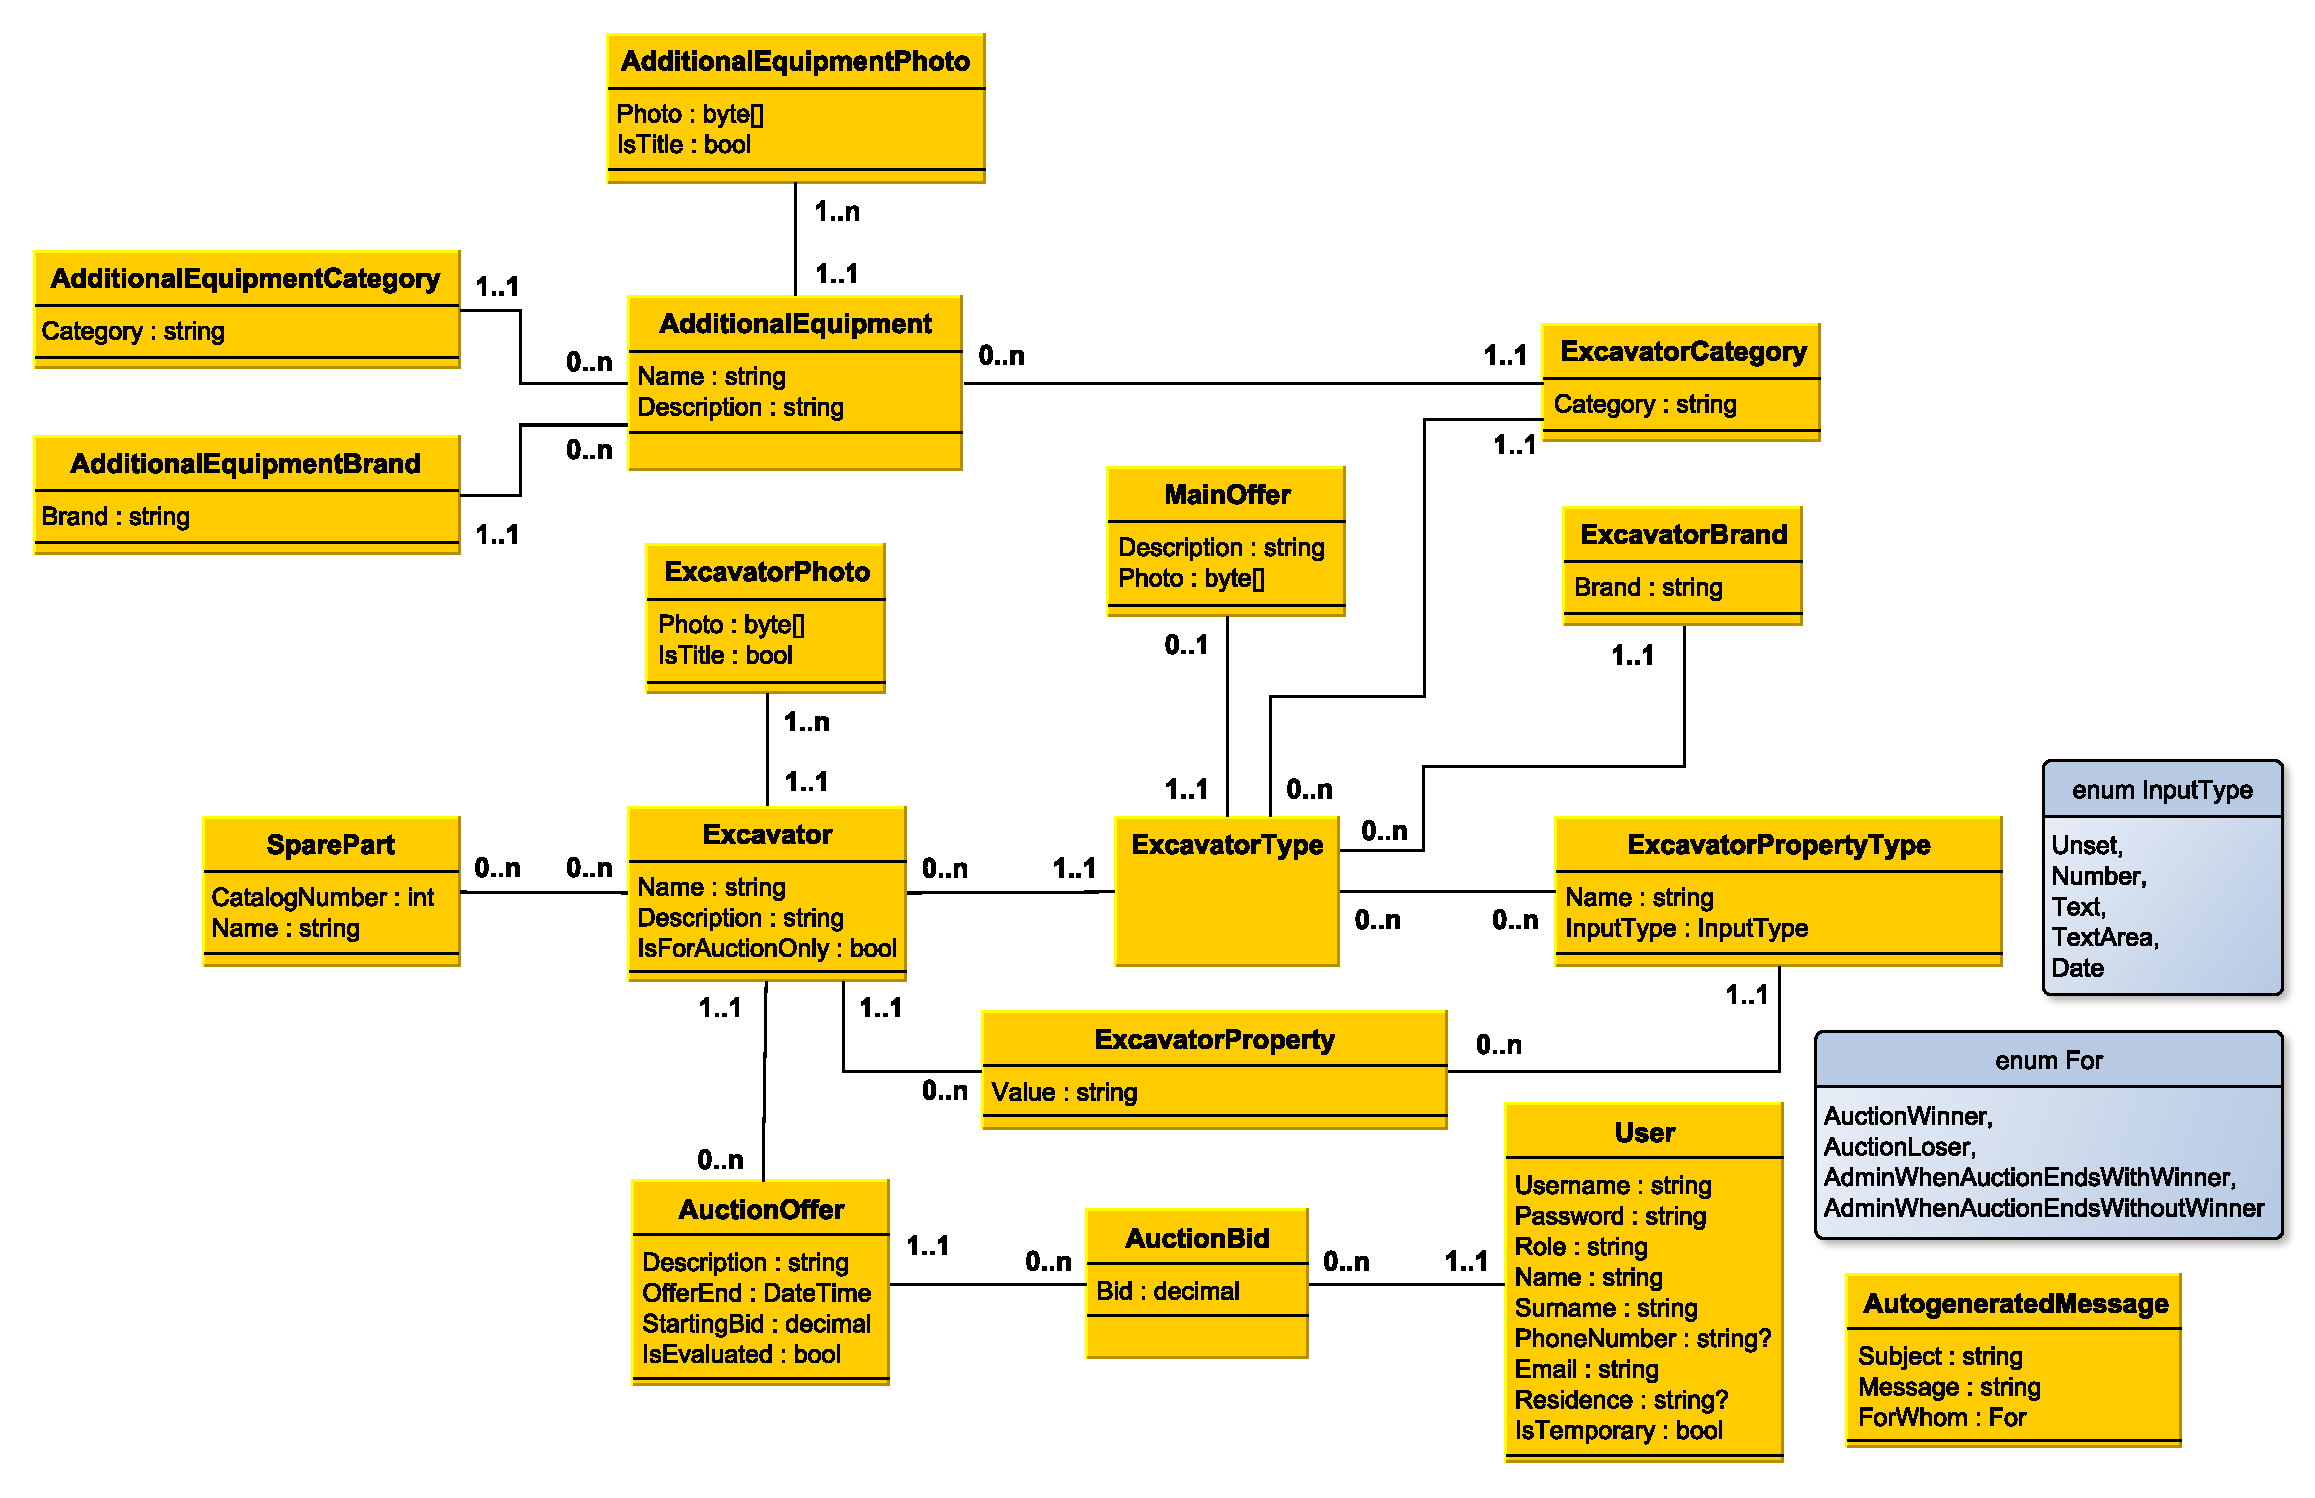
\includegraphics[width=140mm]{../img/relacny model uml}
\caption{Relačný model databázy.}
\label{relacny model uml}
\end{figure}

\begin{itemize}
\item \textbf{Entita Excavator}

V požiadavke P2.2 (Bager, viď~podkap.~\ref{poziadavky}) je napísané, že každý bager má mať názov, značku, kategóriu, opis, fotky, vlastnosti, a~tiež informáciu o~tom, aké náhradné diely obsahuje. Taktiež tam bolo napísané, že môžu existovať bagre, ktoré sú určené iba pre aukciu. To, či je bager určený iba pre aukciu, vieme zachytiť pomocou boolovskej vlastnosti (viď~entitu~Excavator na~obr.~\ref{relacny model uml}). Podobne vieme pomocou vlastností v entite zachytiť aj názov a opis.

\item \textbf{Entita ExcavatorType}

Čo sa týka značky a~kategórie, tak tie by by sme takisto mohli v~entite reprezentujúcej bager zachytiť pomocou vlastností, ale to by znamenalo, že za~každým pri~vytváraní nového záznamu pre bager by sa musela špecifikovať hodnota týchto vlastností. Takisto platí, že viacero bagrov môže byť tej istej kategórie a~značky. Ak by sa mali pri každom vytváraní záznamu bagra vypisovať hodnoty pre značku a kategóriu, mohlo by to viesť k~zbytočným chybám (preklepom), a takisto by to pre administrátora nebolo príliš pohodlné. Preto vytvoríme novú entitu reprezentujúcu typ bagra (viď~ExcavatorType na~obr.~\ref{relacny model uml}), ktorá nám bude určovať kategóriu a~značku bagra. Tato entita však nebude obsahovať vlastnosi ani pre~značku bagra, ani pre~kategóriu bagra.

\item \textbf{Entita ExcavatorBrand a ExcavatorCategory}

Značka bagra, rovnako ako aj kategória bagra, by mali byť novými osobitnými entitami (viď~entity~ExcavatorBrand a~ExcavatorCategory na~obr.~\ref{relacny model uml}), entita reprezentujúca značku bagra by obsahovala vlastnosť s~údajom o~značke bagra a~entita reprezentujúca kategóriu bagra by obsahovala vlastnosť s~údajom o~kategórii bagra. To je z toho dôvodu, že môžu existovať viaceré typy bagra, ktoré by boli rovnakej značky, ale líšili by sa kategóriou (alebo naopak, boli by rovnakej kategórie, ale líšili by sa značkou). Tým, že by sme zo~značky bagra a~kategórie bagra spravili samostatné entity, zamedzili by sme opakujúcim sa hodnotám v~databáze. Takisto kvôli tomuto bude stačiť ak si administrátor v~aplikácii uloží značku (resp.~kategóriu) bagra iba raz, čo môže zamedziť zbytočným chybám (preklepom).

\item \textbf{Entita ExcavatorPhoto}

Tiež boli v súvislosti s bagrami spomenuté fotky bagrov~-- a~tie budú našou ďalšou entitou (viď entitu ExcavatorPhoto na~obr.~\ref{relacny model uml}). Každý bager môže mať viacero fotiek, pričom tieto fotky budeme chcieť zobrazovať napr. v časti aplikácie s detailom bagra, ktorá bola spomenutá v~časti~\ref{detail bagra pridavneho zariadenia} (viď vľavo hore na~obr.~\ref{detail}) alebo~tiež na kartách strojov, ktoré boli spomenuté v~časti~\ref{ponuka novych bagrov} (viď~obr.~\ref{excavator cards}). Entita reprezentujúca fotku bagra by mala okrem samotnej fotky obsahovať aj boolovskú vlastnosť určujúcu, či je fotka titulná. Vďaka tejto vlastnosti budeme môcť presne určiť, aká fotka bagra sa má zobrazovať na~jeho karte.

\item \textbf{Entita SparePart}

Okrem fotiek boli v súvislosti s bagrami spomenuté aj náhradné diely. Náhradný diel bude predstavovať ďalšiu entitu (viď~entitu SparePart na~obr.~\ref{relacny model uml}) a~jeho údaje boli definované v~P7.1~-- má obsahovať katalógové číslo (ide o~celé číslo, neobsahuje iné znaky ako číslice) a~názov náhradného dielu. Každý bager môže obsahovať viacero rôznych náhradných dielov a~jeden náhradný diel sa môže nachádzať vo~viacerých bagroch.

\item \textbf{Entita ExcavatorPropertyType a ExcavatorProperty}

Ďalej boli v súvislosti s bagrami spomenuté aj vlastnosti bagra, ktoré sú určené jeho typom (ako bolo spomenuté v~požiadavke~P2.2). Tu je dôležité uvedomiť si, že typ bagra v skutočnosti určuje typ vlastnosti bagra. Napríklad typ bagra X môže mať vlastnosť hmotnosť a ďalší typ bagra Y môže mať takisto vlastnosť hmotnosť, ale okrem nej môže mať aj vlasnosť šírka lyžice. Všimnime si, že hovoríme o typoch vlastností bagra, ale nie o~konkrétnych hodnotách vlastností, teda napr. koľko vážia bagre typu X, to nemôžeme vedieť, pretože presná hodnota je určená konkrétym bagrom a nie jeho typom. Z toho vyplýva, že budeme potrebovať entitu na reprezentáciu typu vlastnosti bagra (viď entitu ExcavatorPropertyType na obr. \ref{relacny model uml}), ale takisto aj entitu reprezentujúcu (konkrétnu) vlastnosť, ktorá by v sebe niesla konkrétnu hodnotu určenú konkrétnym bagrom (viď entitu ExcavatorProperty na obr. \ref{relacny model uml}). Entita reprezentujúca typ vlastnosti bagra by v sebe mala obsahovať okrem názvu (aby sme vedeli, čo je to za vlastnosť, napr. hmotnosť) aj typ hodnoty danej vlastnosti, aby sme vedeli, či ide o číslo, krátky text, dlhší opis alebo~dátum (s~určením typu hodnoty danej vlastnosti nám pomôže enum~InputType, ktorý môžeme vidieť na~obr.~\ref{relacny model uml}). Tento údaj nám dovolí zlepšiť užívateľské rozhranie, konkrétne typy polí pre hodnoty vlastností bagra vo formulári pre vytvorenie/úpravu bagrov, ktorý bol spomenutý v časti \ref{vytvorenie noveho a uprava existujuceho bagra} (viď obr. \ref{excavator form}).

\item \textbf{Entita MainOffer}

V požiadavke P2 sa vyžaduje, aby existovala aj hlavná ponuka~-- tá bude našou ďalšou entitou (viď entitu MainOffer na obr. \ref{relacny model uml}). Konkrétne v požiadavke P2.1 je napísané, že hlavná ponuka reprezentuje typ bagrov a má obsahovať opis, a tiež fotku danéhu typu. V predošlom texte bolo spomenuté, že môžu existovať bagre, ktoré by boli určené iba pre aukciu, a~teda nenachádzali by sa v ponuke (nových) bagrov. Preto môže nastať situácia, kde by sme chceli, aby sa v databáze nachádzal typ bagra, ale~nechceme, aby existovala v databáze hlavná ponuka pre tento typ bagra. Zároveň platí, že hlavná ponuka predstavuje bagre jedného typu.

\item \textbf{Entita AdditionalEquipment}

V požiadavke P2 je tiež spomenutá aj ponuka prídavných zariadení, preto si vytvoríme aj entitu pre reprezentáciu prídavného zariadenia (viď entitu AdditionalEquipment na obr. \ref{relacny model uml}), tá má podľa požiadavky~P2.3 obsahovať názov, opis, fotky, značku a~kategóriu prídavného zariadenia, ale takisto aj údaj o tom, pre akú kategóriu bagrov je prídavné zariadenie určené. Z~rovnakého dôvodu prečo sme vytvorili novú entitu pre~kategóriu bagra (entita ExcavatorCategory, ktorá bola spomenutá v~prechádzajúcom texte), vytvoríme aj entity reprezentujúce značku prídavného zariadenia (viď~entitu~AdditionalEquipmentBrand na~obr.~\ref{relacny model uml}) a~kategóriu prídavného zariadenia (viď~entitu~AdditionalEquipmentCategory na~obr.~\ref{relacny model uml}). Ďalej čo sa týka fotiek prídavného zariadenia, tak by sa naskytovala možnosť zmeniť entitu reprezentujúcu fotky bagrov (ExcavatorPhoto) na~entitu reprezentujúcu fotky všeobecne (aj bagrov, aj prídavných zariadení). No~tento prístup by nám umožnil priradiť fotku prídavného zariadenia bagru (a~naopak), čo nie je správne. Preto namiesto toho vytvoríme, rovnako ako v~prípade fotky bagra, novú entitu reprezentujúcu fotku prídavného zariadenia (viď~entitu~AdditionalEquipmentPhoto na~obr.~\ref{relacny model uml}).

\item \textbf{Entita User}

Ďalej z požiadavky P6 vieme, že budeme potrebovať entitu reprezentujúcu užívateľa (viď~entitu~User na~obr.~\ref{relacny model uml}). Konkrétne z~P6.3 vieme, že o užívateľovi potrebujeme vedieť jeho prihlasovacie meno, heslo, (krstné) meno, priezvisko, email, príp.~aj telefónné číslo a~bydlisko (mesto). No okrem týchto údajov sa nám tiež kvôli požiadavke P6.1 hodí údaj, či je užívateľ dočasný. Presnejšie je to kvôli tomu, aby aj neprihlásený užívateľ mohol ponúkať sumy do dražby. Po ponúknutí sumy by sa do~databázy uložila informácia o tom, kto ponúkol sumu (a~tiež čo to bolo za~aukčnú ponuku). Po prejdení termínu konca aukčnej ponuky a~vyhodnotení aukcie sa budú môcť tieto dočasné účty vymazať. Okrem toho by sa nám tiež hodil údaj o~tom, či je užívateľ bežným zákazníkom alebo~administrátorom, aby mu podľa toho vedel systém zobraziť správny obsah (vychádza z~P1~Roly užívateľa, viď~podkap.~\ref{poziadavky}). Všetky tieto údaje by mali byť zahrnuté vo~vlastnostiach entity User.

\item \textbf{Entita AuctionOffer}

Z požiadavky P4 vieme, že administrátor by mal byt schopný zaradiť bager do~aukcie a~vytvoriť tak aukčnú ponuku~-- to bude našou ďalšou entitou (viď~entitu~AuctionOffer na~obr.~\ref{relacny model uml}). Takisto z~požiadavky P4 vieme, že administrátor by mal mať možnosť zadať dátum konca aukčnej ponuky, počiatočnú sumu a~popis ponuky (v~ňom môže byť napísané napr.~čo bolo v~bagri opravené). Preto budú tieto údaje vlastnosťami entity~AuctionOffer.

\item \textbf{Entita AuctionBid}

Okrem entity AuctionOffer vyplýva z požiadavky P4 aj entita reprezentujúca ponuku (sumu) ponúknutú zákazníkom (viď~entitu~AuctionBid na~obr.~\ref{relacny model uml}). Údaj o tom, koľko zákazník ponúkol, je vlastnosťou entity~AuctionBid.

\item \textbf{Entita AutogeneratedMessage}

Našou poslednou entitou bude entita pre~automaticky generované správy, ktorej potreba vyplýva z~požiadaviek~P4.1 a~P5.3. Z~P4.1 vieme, že budeme potrebovať odosielať automaticky generované správy~-- konkrétne budeme potrebovať odosielať správy víťazom dražieb, porazeným, ale~takisto aj administrátorom v~prípade, že dražba skončila (a~to aj v prípade, že skončila bez víťaza). Všetky tieto prípady zachytáva enum~For, ktorý môžeme vidieť na~obr.~\ref{relacny model uml}. Ďalej z~P5.3 vieme, že chceme dovoliť administrátorom upravovať formát automaticky generovaných správ, preto potrebujeme entitu reprezentujúcu automaticky generovanú správu (viď~entitu~AutogeneratedMessage na~obr.~\ref{relacny model uml}). V~požiadavke~P4.1 je napísané, že sa tieto automaticky generované správy majú posielať ako emaily, preto by mala entita~AutogeneratedMessage obsahovať vlastnosti pre~predmet a~samotný text správy. Tiež by mala obsahovať vlastnosť určujúcu pre~koho, resp.~pre~akú príležitosť, je automaticky generovaná správa určená.

\end{itemize}

\subsection{Voľba databázového servera}

Čo sa týka databázového servera, tak si najprv poďme rozmyslieť, čo od~neho budeme vyžadovať. Kvôli požiadavke P11 (Náklady, viď~podkap.~\ref{poziadavky}) chceme, aby bol server (v~najlepšom prípade) bezplatný. Taktiež musí byť kompatibilný s~platformou .NET. Tieto požiadavky spĺňajú servery: \href{https://www.microsoft.com/en-us/sql-server/sql-server-2022-comparison}{Microsoft SQL Server (Express edition)}, \href{https://www.oracle.com/database/technologies/appdev/xe.html}{Oracle Database (Express edition)} a~\href{https://dev.mysql.com/downloads/mysql/}{MySQL (Community server)}. V~prípade prvých dvoch serverov je síce pravda, že poskytujú aj bezplatnú verziu, ale sú obmedzené na~kapacitu (pri serveri Microsoft SQL je to 10~GB, pri Oracle Database je to 12~GB). Síce je pravda, že aj napriek obmedzeniu je kapacita pre naše účely (pre malé firmy) dostatočne veľká, ale v~prípade Community verzie MySql takéto obmedzenie kapacity nemáme žiadne. V~budúcnosti, ak by sa firme darilo a~získala by viacej zákazníkov, prípadne rozšírila ponuku, by sa nám mohla neobmedzená kapacita servera hodiť. Preto si volíme MySql.

\subsection{Object Relational Mapping}

\href{https://www.freecodecamp.org/news/what-is-an-orm-the-meaning-of-object-relational-mapping-database-tools/}{Object Relational Mapping (ORM)} je technika využívaná pri prepájaní \href{https://www.freecodecamp.org/news/four-pillars-of-object-oriented-programming/}{objektovo orientovaného programovania (OOP)} a (vo väčšine prípadov) relačných databáz. Pri~práci s~relačnou databázou môžeme vytvárať, čítať, editovať a mazať dáta z~databázy pomocou jazyka SQL (SQL skripty), ale~takisto môžme využiť ORM nástroje pre~uľahčenie práce. Populárnymi ORM nástrojmi na~platforme~.NET sú napr.~frameworky Dapper alebo~Entitity Framework Core (ďalej už len EF Core).

Ako bolo spomenuté, v našom programe by sme mohli využiť pre~prácu s~databázou (\uv{čisté}) SQL skripty. Výhodou tohto prístupu je väčšia kontrola nad~SQL dotazmi, a~rýchlosť vykonania dotazov. Nevýhodou je, že tento prístup nám neposkytuje automatické \href{https://www.linkedin.com/advice/0/how-do-you-handle-user-input-validation-sanitization}{sanitizovanie dotazov}, a takisto neposkytuje dopĺňanie kódu (nápovedu) ako napr.~pri~C\# kóde vo~Visual Studiu. Navyše je tento prístup dosť pracný, a~to v~tom zmysle, že by sme museli napísať veľa SQL kódu už len pre vytvorenie tabuliek. Alternatívou by bolo využitie nejakého ORM frameworku, napr.~Dapper alebo~EF Core, tento prístup by nám poskytol automatické dopĺňanie kódu vo~Visual Studiu, pretože by sme pracovali so~C\# kódom. Obe frameworky si teraz porovnáme. 

Dapper je jednoduchším frameworkom oproti frameworku EF Core s~menším počtom funkcionalít. Umožňuje spúšťať SQL dotazy a ich výsledky mapovať na~.NET objekty. Výhodou naďalej ostáva kontrola nad~tvarom dotazu a~rýchlosť vykonania dotazu, pretože stále pracujeme s~dotazmi napísanými jazykom~SQL. Ale naďalej ostáva nevýhodou, že by sme museli pracne pomocou jazyka SQL vytvárať všetky tabuľky.

EF Core je mohutnejší ORM framework s viacerými funkcionalitami. Jeho nevýhodou oproti predošlým možnostiam je, že vykonávanie dotazov je pomalšie, no stále ide o rozumné časy, ktoré pre~nás nepredstavujú problém (viac o~časovej výkonnosti spomínaných možností je možné nájsť \href{https://github.com/DapperLib/Dapper\#performance}{tu} alebo~aj \href{https://levelup.gitconnected.com/dapper-vs-ef-core-which-orm-framework-should-you-choose-for-your-net-application-54f2723b176a}{tu}). Oproti predošlým možnostiam nám však umožňuje využiť prístup \href{https://www.entityframeworktutorial.net/code-first/what-is-code-first.aspx}{code first} pri~vytváraní tabuliek. Tento prístup nám umožní zamerať sa na~doménu našej aplikácie, pričom bude stačiť vytvoriť pomocou C\# kódu (doménové) modely (ide o~C\# triedy predstavujúce entity vytvorené v~časti~\ref{navrh relacneho modelu databazy}), a z~nich si pomocou frameworku EF Core budeme schopný nechať vygenerovať SQL kód a~vytvoriť tabuľky bez toho, aby sme museli manuálne písať SQL skripty. To nám môže potenciálne zjednodušiť a~urýchliť implementáciu systému. Preto si zvolíme ako ORM framework~EF Core. Viac informácií o~frameworkoch Dapper a~EF Core je možné nájsť \href{https://www.c-sharpcorner.com/article/dapper-vs-entity-framework-core/}{tu}.

\section{Aukcia- odpočet a vyhodnocovanie}
\label{aukcia odpocet a vyhodnocovanie}

V požiadavke P4.2 (Odpočet a ďalšie údaje, viď~v~podkap.~\ref{poziadavky}) sa vyžaduje odpočet do~konca dražby. Túto požiadavku by sme splnili implementáciou častí aplikácie navrhnutých v častiach textu \ref{aukcne ponuky} (Aukčné ponuky, odpočet by sa nachádzal v spodnej časti vylistovaných kariet, viď obr. \ref{auction offer cards}) a~\ref{detail aukcnej ponuky} (Detail aukčnej ponuky, odpočet by sa nachádzal v~texte so~základnými informáciami, viď vpravo hore na~obr.~\ref{auction offer detail}). V tejto podkapitole si rozoberieme ako by sme mohli implementovať odpočet (a aj vyhodnocovanie aukčných dražieb) v~spomínaných častiach aplikácie.

Keďže každá zo spomínaných častí aplikácie zobrazuje informácie o~aukčnej ponuke, musí mať prístup k~entite~AuctionOffer, ktorú sme si zadefinovali v~časti~\ref{navrh relacneho modelu databazy}. Táto entita obsahuje okrem iného aj dátum, kedy končí aukčná ponuka. Ak od neho odčítame aktuálny dátum a~čas (pomocou \verb|DateTime.Now|), tak získame koľko času ostáva do~konca aukčnej ponuky a tento údaj môžeme zobraziť užívateľovi. Lenže to nám nestačí, pre~odpočet budeme potrebovať, aby sa nový údaj zobrazil každú sekundu. Na to by sme mohli využiť \href{https://learn.microsoft.com/en-us/dotnet/api/system.timers.timer?view=net-6.0}{triedu \texttt{Timer}}, ktorú nám platforma .NET ponúka. Po prejdení určitého intervalu (ktorý si vieme zadať pri vytvorení inštancie) vygeneruje udalosť. Takže ak si nastavíme interval jednu sekundu a zaregistrujeme si metódu, ktorá by prepočítala čas do konca aukčnej ponuky a prekreslila údaj na stránke, tak dosiahneme požadovaného odpočtu.

Implementácia by mohla byť realizovaná tak, že by pre~každé miesto s~odpočtom existovala jedna inštancia triedy~\verb|Timer|. To by však znamenalo mrhanie zdrojmi (viac informácií \href{https://learn.microsoft.com/en-us/dotnet/api/system.threading.timer.dispose?view=net-6.0}{tu}). Lepším riešením by bolo vytvoriť službu (triedu, ktorá by sa mohla volať napr.~\verb|EverySecondTimerService|), ktorá by nám dovolila registrovať ľubovoľné metódy (v~našom prípade metódy pre~prepočítanie a~prekreslenie odpočtu) a~každú sekundu by zavolala registrované metódy. Potom by nám stačilo vytvoriť jednu inštanciu spomínanej služby, ktorá by využívala jednu inštanciu triedy~\verb|Timer| a~pomocou \href{https://learn.microsoft.com/en-us/aspnet/core/blazor/fundamentals/dependency-injection}{dependency injection}, ktorý je vstavaný vo~frameworku~Blazor Server, si vyžiadať inštanciu triedy~\verb|EverySecondTimerService| z~každého miesta s~odpočtom v~aplikácii podľa potreby.

Triedu \verb|Timer| by sa nám tiež hodilo využiť aj pre~vyhodnocovanie dražieb. Povedzme, že napr. každú minútu by systém prešiel všetky aukčné ponuky, ktoré by už neboli aktívne (t.~j.~prešiel ich termín konca) a~pre~každú z aukčných ponúk by sa zistilo, ktorý užívateľ ponúkol najvyššiu sumu a~oboznámime ho, že vyhral. Taktiež by systém oboznámil ostatných účastníkov dražby s tým, že dražbu nevyhrali, a~takisto by boli oboznámil aj administrátorov, že dražba skončila (a~to aj v prípade, že skončila bez~víťaza). Trieda, ktorá by bola zodpovedná za tento proces by sa mohla volať napr.~\verb|AuctionEvaluatorService|.

Zároveň si všimnime, že tu už máme dve triedy (\verb|EverySecondTimerService| a~\verb|AuctionEvaluatorService|), ktoré by využívali triedu~\verb|Timer|. Obe chcú zadať interval (v~prípade \verb|EverySecondTimerService| ide o sekundu, v prípade \verb|AuctionEvaluatorService| ide o minútu) a~špecifikovať čo sa má diať (napr.~pomocou \verb|AuctionEvaluatorService| chceme každú minútu skontrolovať aukčné ponuky a~v~prípade potreby ich aj vyhodnotiť). Aby sme zamedzili duplicitnému kódu, tak by sme mohli vytvoriť rodičovksú triedu~\verb|TimerService| (viď~obr.~\ref{timer services uml}), ktorá by pokryla túto spoločnú logiku.

\begin{figure}[H]\centering
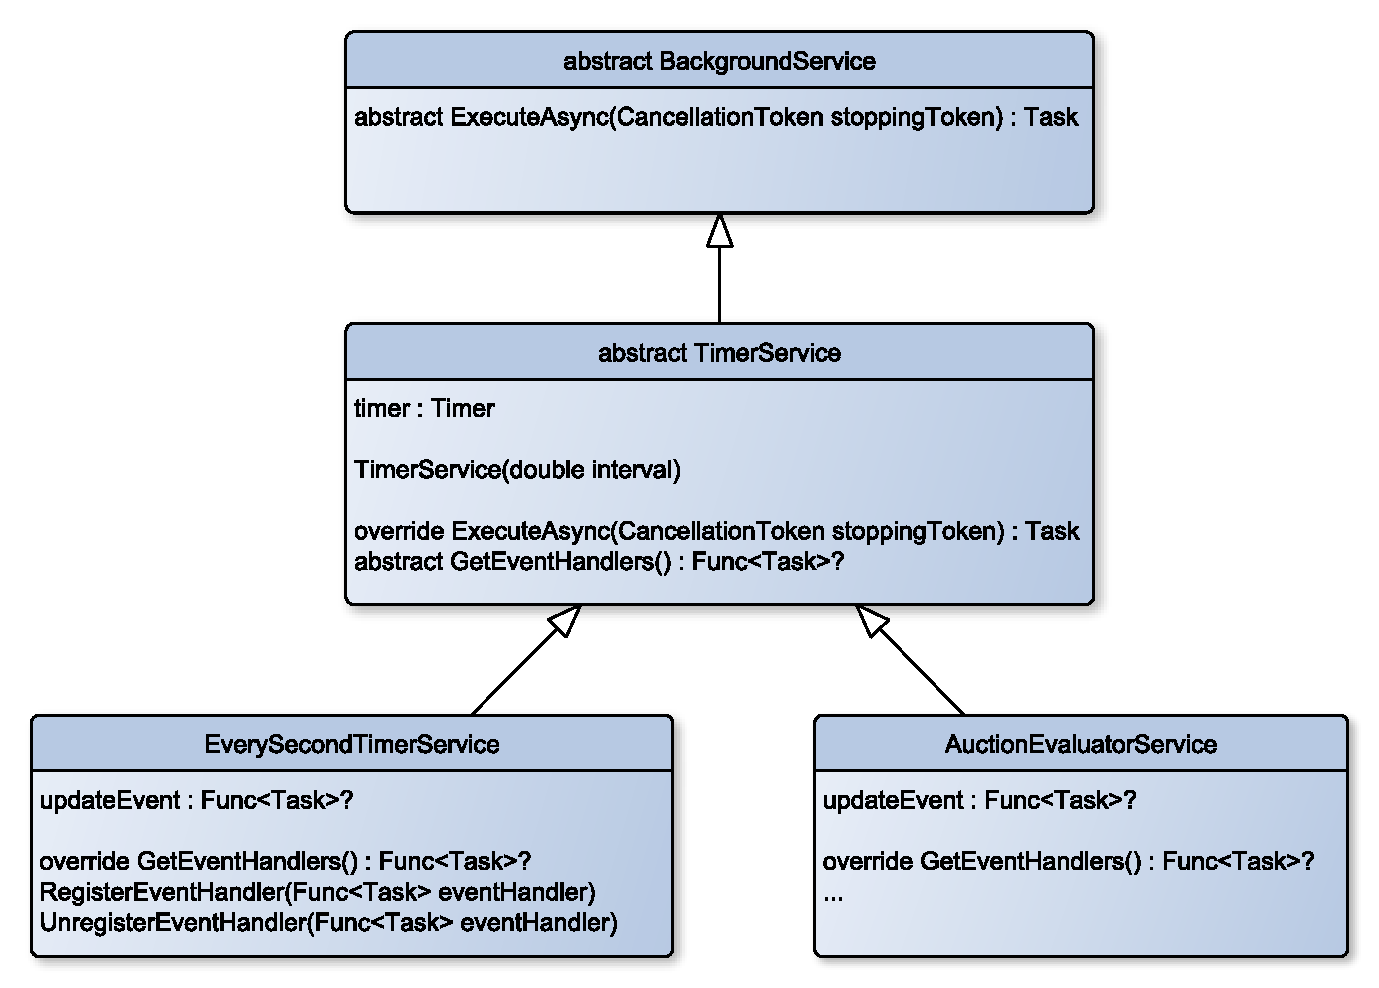
\includegraphics[width=140mm]{../img/timer services uml}
\caption{Časové služby využívajúce triedu \texttt{Timer}.}
\label{timer services uml}
\end{figure}

Interval by sa mohol predať potomkami prostredníctom parametra konštruktora triedy~\verb|TimerService| a pomocou abstraktnej metódy \verb|GetEventHandlers| triedy~\verb|TimerService| by si potomkovia mohli zadefinovať čo sa má diať. Takže v prípade triedy \verb|EverySecondTimerService| by to bolo prepočítanie a~prekreslenie odpočtu (resp.~zavolanie registrovaných metód) a v prípade triedy \verb|AuctionEvaluatorService| by to bolo prejdenie aukčných ponúk a~vyhodnotenie tých ktoré by boli neaktívne.

Ďalej je potrebné si uvedomiť, že kód oboch služieb (\verb|EverySecondTimerService| a~\verb|AuctionEvaluatorService|) musí bežať na~pozadí v~osobitnom vlákne, aby neblokoval program a~neznepríjemňoval tým užívateľovi prácu s~aplikáciou. Pre implementáciu kódu bežiaceho na~pozadí nám .NET poskytuje viacero možností, pre naše účely by sa hodili napr. rozhranie \href{https://learn.microsoft.com/en-us/aspnet/core/fundamentals/host/hosted-services?view=aspnetcore-7.0&tabs=visual-studio\#ihostedservice-interface}{\texttt{HostedService}} alebo trieda \href{https://learn.microsoft.com/en-us/aspnet/core/fundamentals/host/hosted-services?view=aspnetcore-7.0&tabs=visual-studio\#backgroundservice-base-class}{\texttt{BackGroundService}}. Pre naše účely by sa dali využiť obe možnosti, no trieda~\verb|BackGroundService| je určená pre~dlhotrvajúce úlohy bežiace na~pozadí (viac informácií \href{https://www.compositional-it.com/news-blog/background-tasks-in-net}{tu}), navyše autorovi vyhovuje viac možnosť s~triedou \verb|BackGroundService|, preto použijeme túto možnosť, a~to tak, že trieda \verb|TimerService| bude dediť od~triedy~\verb|BackGroundService|.

Trieda \verb|TimerService| zdedí od triedy \verb|BackGroundService| abstraktnú metódu \href{https://learn.microsoft.com/en-us/dotnet/api/microsoft.extensions.hosting.backgroundservice.executeasync?view=dotnet-plat-ext-7.0\#microsoft-extensions-hosting-backgroundservice-executeasync(system-threading-cancellationtoken)}{ExecuteAsync}. V~triede \verb|TimerService| by sme ju mohli naimplementovať tak, že poz zavolaní by sa inicializovala inštancia triedy~\verb|Timer|, na ktorej by sa zavolala metóda \href{https://learn.microsoft.com/en-us/dotnet/api/system.timers.timer.start}{\texttt{Start}}). Inicializácia by spočítavala v~tom, že na udalosť \href{https://learn.microsoft.com/en-us/dotnet/api/system.timers.timer.elapsed}{Elaped} inštancie triedy \verb|Timer| by sa zaregstrovali metódy (obsluhy udalostí) definované v potomkoch, tie vieme získať pomocou metódy \verb|GetEventHandlers| (ktorú sme spomenuli skôr v~texte). Ďalej nám už len stačí registrovať služby \verb|EverySecondTimerService| a~\verb|AuctionEvaluatorService| pomocou metódy \verb|AddHostedService| (viac informácii \href{https://learn.microsoft.com/en-us/dotnet/core/extensions/timer-service?pivots=dotnet-7-0}{tu}). Potom po~spustení aplikácie a~registrácií služieb sa už framework postará o~zavolanie našej implementácie metódy \verb|ExecuteAsync| (a~tým spustí na~pozadí naše služby).

%\section{Zmena UI podla Roly}

%TODO?

%\section{Posielanie a prijimanie sprav}

%TODO?

%\subsection{Injectovanie vlastnych dat, napr url do emailov}

%TODO? (do spravy je problem lebo by videl uzivatel, do headru je ok)

%\subsection{Posielanie automaticky generovanych sprav, resp tvorba sablon}

%TODO? (default spravy by mohli byt v db ale to by sa vymazali kebyze sa raz prepisu, mohli by byt v roznych stlpcoch sice ale nechcel som pridavat do db aby sa nezvysoval cost za db... asi som to mohol radsej tak spravit no...)

%\section{Management, data grid od Syncfusionu}

%TODO?

\iffalse

---

PO TADE JE NOVY TEXT

---

\section{Aukcia- odpočet a vyhodnocovanie}

Ako už bolo skôr v~texte spomenuté, budeme potrebovať nejaký mechanizmus, ktorý zvládne vykonávať odpočet do~konca každej aukčnej ponuky, a~takisto aby ju po~skončení vedel vyhodnotiť.

Odpočet by sme mohli implementovať tak, že by sme si vytvorili inštanciu triedy \verb|Timer|\footnote{\url{https://learn.microsoft.com/en-us/dotnet/api/system.timers.timer?view=net-8.0}} pre~každú aukčnú ponuku. Každá z~inštancií by každú sekundu odpálila event, pri~ktorom by došlo k~prerenderovaniu komponentu s~časom do~skončenia ponuky. Toto riešenie by síce fungovalo, ale je to mrhanie zdrojmi. Stačí nám jeden \verb|Timer|. Na~jeho event \verb|Elapsed| si každý komponent s~odpočtom zaregistruje metódu na~prerenderovanie. Týmto spôsobom sa nám podarí ušetriť zdroje, ale vyskytá sa otázka. Kde bude inštancia triedy \verb|Timer| uložená? Prirodzenou odpoveďou by bolo, že ju uložíme do~rodičovského komponentu. Limitácia tohto riešenie spočíva v~tom, že ak budeme potrebovať vykonať nejakú operáciu periodicky každú sekundu, ale v~komponente, ktorá sa nenachádza v~rodičovi s~triedou \verb|Timer|, tak nemáme prístup k~triede \verb|Timer|. Lepším riešením bude presunúť \verb|Timer| do~nového vlákna, ktoré bude bežať na~pozadí. Takýmto spôsobom si môžeme kedykoľvek a~odkiaľkoľvek registrovať periodické operácie.

Tu by som sa ešte rád zastavil a vrátil k~poznámke z~úvodu, kedy som spomenul, že komponenty nám pomôžu vyriešiť problém s~odpočtom. Vieme, že kvôli odpočtu dôjde každú sekundu k prerenderovaniu stránky. No určite nechceme, aby sa nám každú sekundu prerenderovávala celá stránka (resp.~hľadali zmeny na~celej stránke). Ak izolujeme odpočet do~samostatného komponentu, prerenderovanie sa vykoná iba v~ňom. Zbytok stránky to neovplyvní.

Ďalej si potrebujeme rozmyslieť ako bude prebiehať vyhodnocovanie aukcie. Náš systém bude fungovať tak, že užívateľ (ak má záujem o~dražený stroj) odošle svoju~ponúkanú sumu. Tá sa uloží v~databáze. Potrebujeme mechanizmus, ktorý by sledoval aukčné ponuky. Ak by uvidel, že nejaká z~ponúk už skončila, tak ju vyhodnotí. Periodické sledovanie aukčných ponúk je dlhodobo bežiaca operácia, a~preto sa hodí ju takisto vykonávať vo~vedľajšom vlákne na~pozadí.

Poďme sa ešte pozrieť na~to, čo presne zahŕňa vyhodnocovanie jednej aukčnej ponuky. Prejdeme všetky ponúknuté sumy, nájdeme najvyššiu sumu a~užívateľ, ktorý ju ponúkol bude vyhlásený za~víťaza. Víťaz aukcie bude informovaný o~skutočnoti, že vyhral stroj v~aukcii. Porazení budú takisto oboznámení o~svojej prehre. Okrem tohto scenára existuje ešte jeden. Čo ak sa nikto nezapojil do~aukcie? Má sa aukčná ponuka zmazať? Alebo iba označiť za~ukončnenú a~schovať sa pred~bežnými zákazníkmi? Alebo sa má koniec aukcie presunúť na~neskôr? Ako vidíme možností je viacero. Prvé dve možnosti vyžadujú zásah admina, ktorý by musel nanovo vložiť ponuku do systému~(prvý prípad) alebo~upraviť ponuku a~znova ju zviditeľniť zákazníkom~(druhý prípad). Všimnime si, že posledná z~možností nevyžaduje akciu admina. Administrátor môže ponuku upraviť, ale nemusí. Systém sa postará sám o~seba a~funguje aj bez~zásahu admina. A~to je presne to, čo od~nás vyžuje P3. Preto volíme tretí prístup. V~prípade, že aukcia skončí bez~víťaza, tak systém o~tom upozorní administrátora a~koniec ponuky posunie na~neskôr~(napr. o~týždeň).

V~oboch prípadoch (odpočet i~vyhodnocovanie) sme sa rozhodli využiť vlákna na~pozadí. Vo~frameworku Blazor existuje trieda~\verb|BackgroundService|\footnote{\url{https://learn.microsoft.com/en-us/aspnet/core/fundamentals/host/hosted-services?view=aspnetcore-7.0&tabs=visual-studio\#backgroundservice-base-class}}. Tá nám umožní rozbehnúť kód na~pozadí. Takže logiku behu vlákien na~pozadí si nemusíme implementovať sami.

\section{Posielanie a prijímanie správ}

Dospeli sme k~tomu, že nepotrebujeme správy len odosielať ale potrebujeme ich aj čítať. Ešte predtým, než si zvolíme spôsob akým budeme správy prijímať a~posielať, si poďme vybrať akú emailovú službu budeme využívať. Od~služby vyžadujeme, aby podporovala protokoly IMAP~(pre~prijímanie správ) a~SMTP~(pre~posielanie správ). Jednou zo~služieb ktorá spĺňa podmienku je Gmail od~spoločnosti Google. Ide o~veľkú spoločnosť, ktorú pozná snáď každý a~autor dôveruje ich zabezpečeniu. Ďalším plusom je to, že k~tejto službe existuje dokumentácia. Navyše služba poskytuje API~(z~ang. application programming interface), ktoré by sme mohli využiť v~prípade potreby. Čítateľ by mohol poznamenať, že API by sme mohli vyyužiť ku~kompletnej implementácii našej schránky. Dôvodom prečo nevyužijeme API služby pre~kompletnú implementáciu je ten, že to čo ideme vytvoriť sa skôr podobá emailovému klientovi. Na~jeho implemenáciu je vhodnejšie použiť protokoly~IMAP a~SMTP ~(rovnako to spomína i~dokumentácia API\footnote{\url{https://developers.google.com/gmail/api/guides}}). Ako vidíme, Gmail sa zdá byť dobrým kandidátom, a~preto si ho zvolíme.

Ďalej potrebujeme zistiť ako môžeme využívať protokoly IMAP a~SMTP z~nášho programu. Zdá sa, že najznámejšími balíčkami pre~prácu s~týmito protokolmi sú MailKit a~AE.Net.Mail. Obe umožňujú prácu s~IMAP i~SMTP, ale AE.Net.Mail nebol už dlhšiu dobu aktualizovaný. A~preto, ak sa z~tohto systému stane dlhodobejší projekt, sa zdá byť lepšou možnosťou MailkKit.

%\section{Ďalší kód tretích strán}
%TBA? (Fontawesome, Syncfusion) + pridať že management treba na zaciatok %analyzy (ako do db sa daju veci? Treba inteface pre adminov!)

\fi

\chapter{Vývojová dokumentácia}

V~tejto kapitole sa pozrieme na~implementáciu nášho~systému. Zameráme sa na~organizáciu a~implementáciu dôležitých častí aplikácie. Cieľom tohto textu nie je opísať správanie každého riadku kódu. Na~to slúži kód samotný~(prípadne komentáre, ktoré autor pridal na~miesta, kde to uznal za~vhodné).

Celá aplikácia je rozdelená do~dvoch projektov-~ServISData a~ServISWebApp.

\section{ServISData}

Zmyslom projektu ServISData je správa databázových entít a~komunikácia s~databázou. Teraz si prejdeme jednotlivé priečinky tohto projektu a~popíšeme si ich~obsah.

\subsection{Koreňový priečinok projektu}

Nachádza sa tu \verb|ServISDbContext| a~spolu s~ním i~\verb|ServISDbContextFactory|. Tieto triedy sú zodpovedné za~konfiguráciu databázy, a~tiež samotné pripojenie aplikácie k~databáze. Viac o~týchto triedach a~spôsobu ich použitia v~projekte nájdeme~\href{https://learn.microsoft.com/en-us/ef/core/dbcontext-configuration/\#using-a-dbcontext-factory-eg-for-blazor}{tu}.

V~priečinku sa tiež nachádzajú triedy~\verb|AutogeneratedMessageForExtensions| a~\verb|InputTypeExtensions|. V~oboch prípadoch ide o~extension metódy umožňujúce získať metadáta z~atribútov, ktoré sme použili v~enumoch~\verb|AutogeneratedMessage.For| a~\verb|InputType|.

Takisto sa v~priečinku nachádza už spomenutý~\verb|InputType|. Ide o~enum, ktorého hodnoty predstavujú možné typy hodnôt vlastností stroja.

Ďalej sa tu nachádza trieda~\verb|ServISApi|. Tá slúži pre~komunikáciu s~databázou. Respektíve umožnuje iným projektom~(v~našom prípade ServISWebapp) modely ukladať, čítať, editovať a~mazať z~databázy.

\subsection{Attributes}

Priečinok obsahuje atribúty\footnote{\url{https://learn.microsoft.com/en-us/dotnet/csharp/advanced-topics/reflection-and-attributes/}}. Konkrétne ide o~\verb|AutogeneratedMessageDataAttribute| a~\verb|InputTypeLabelAttribute|.

Prvý slúži na~nastavenie predvoleného predmetu a~textu automaticky generovaných správ, ale takisto aj na~nastavenie ich podporovaných tagov.

Druhý slúži pre~uloženie užívateľsky prívetivejšieho názvu typu hodnoty vlastnosti stroja. Tieto názvy sa zobrazujú napríklad pri~vytváraní typu vlastnosti stroja.

\subsection{DataOperations}

Priečinok obsahuje triedy, ktoré ich~užívateľom umožnia vykonávať rôzne operácie nad~dátami (filtrovanie, stránkovanie,\dots).

\subsection{Interfaces}

Priečinok obsahuje rozhrania~(ang.~interfaces).

\verb|IServISApi| nás zbaví potreby upravovať kód využívajúci API projektu ServISData v~prípade, ak sa rozhodneme vymeniť \verb|ServISApi| za~nejakú inú implementáciu.

\verb|IPhoto| nám umožní všeobecne pracovať s~fotkami aj napriek tomu, že pôjde o~fotky rôznych entít.

\verb|IItem| nám dovolí písať všeobecný kód pre~prácu s~modelmi entít~(využíva sa napr.~pri~mazaní entít z~databázy; viď~metódu~\verb|DeleteItem| v~triede~\verb|ServISApi|).

\subsection{Migrations}

Tento priečinok bol vygenerovaný frameworkom~Entity~Framework~Core a~obsahuje vygenerovaný kód. Ide o~migrácie\footnote{\url{https://learn.microsoft.com/en-us/ef/core/managing-schemas/migrations/?tabs=dotnet-core-cli}}. Nad~migráciou môžeme rozmýšlať ako nad~commitom v~gitu. Po~aplikovaní migrácie dôjde k~zmene v~databáze~(napr.~sa pridá nový stĺpec do~nejakej z~tabuliek).

\subsection{Models}

Priečinok obsahuje modely-~triedy reprezentujúce entity uložené v~databáze.

\section{ServISWebApp}
TBA

\chapter{Užívateľská dokumentácia}

Návod pre zákazníkov ako pracovať s~aplikáciou je možné nájsť v~podobe\linebreak videí na~adrese v~prílohe (viď~\ref{videonavod pre zakaznikov}), takisto je v~prílohe možné nájsť aj videonávody na~používanie aplikácie pre~administrátorov (viď~\ref{videonavod pre administratorov}). Čo sa týka procesov spustenia systému pre~lokálne testovanie a~nasadenia na~internet, tak tie si opíšeme v~tejto kapitole.

\section{Databáza}
\label{databaza}

Aplikácia ServIS využíva pre ukladanie dát databázu~MySQL, ktorá nie je súčasťou aplikácie, a~preto je nutné si ju osobitne stiahnuť a~nainštalovať. Odkaz na~stiahnutie je možné nájsť na~stránkach databázy~\cite{mysql}, rovnako ako aj návod na~inštaláciu~\cite{mysql navod}.

\section{Predpoklady pre lokálne spustenie}
\label{predpoklady}

Pre úspešné nainštalovanie, spustenie a~fungovanie aplikácie budeme potrebovať:

\begin{itemize}
\item Počítač s~operačným systémom Windows~10 alebo~vyššie
\item Prístup na internet
\item Visual Studio 2022~\cite{visual studio} (budeme potrebovať .NET~6 alebo~vyššie)
\item Databáza MySQL (viac v~podkapitole~\ref{databaza})
\end{itemize}

\section{Návod na lokálne spustenie}
\label{navod}

V~tejto podkapitole si povieme ako spustiť aplikáciu lokálne. Návod sa spolieha, že sú splnené všetky predpoklady z~podkapitoly~\ref{predpoklady}, a~takisto na to, že čítateľ už má k dispozícií repozitár aplikácie (jednou z~možností ako získať repozitár aplikácie je stiahnuť si ho z~online repozitára, pre odkaz naň viď prílohu~\ref{implementacia}).

\begin{enumerate}
  \item V priečinku (repozitári) aplikácie si dvojitým kliknutím na~\verb|ServIS.sln| otvoríme aplikáciu v programe Visual Studio 2022.
  \item V \verb|appsettings.json| sa nachádza konfigurácia aplikácie, kde je možné nastaviť napr.~názov firmy, aký má byť minimálny rozdiel medzi ponukami v~aukcii atď. Nastavíme ju podľa svojich údajov (\verb|Logging| a~\verb|AllowedHosts| môžeme ignorovať).
  \newpage
  \item Pravým tlačidlom myšy klikneme na projekt ServISData, a~potom klikneme na~\uv{Manage User Secrets}. Zobrazí sa nám súbor, ktorého obsah by mal vyzerať takto:
  
\begin{verbatim}
{
    "ConnectionStrings": {
        "Default": "CONNECTION_STRING"
    }
}
\end{verbatim}  
  
Namiesto \verb|CONNECTION_STRING| vložíme svoj connection string databázy (stačí ak využijeme štandardný tvar connection stringu~\cite{standard connection string}).

  \item Pravým tlačidlom myšy klikneme na projekt ServISWebApp, a~potom klikneme na \uv{Manage User Secrets}. Zobrazí sa nám súbor, ktorého obsah by mal vyzerať takto:
  
\begin{verbatim}
{
    "SyncfusionLicenseKey": "LICENSE_KEY",
    "EmailAppPassword": "APP_PASSWORD"
}
\end{verbatim}  
  
Namiesto \verb|LICENSE_KEY| vložíme svoj licenčný kľúč (postup získania kľúča je opísaný v~dokumentácii spoločnosti Syncfusion~\cite{license key}). Namiesto \verb|APP_PASSWORD| vložíme svoje emailové heslo aplikácie (postup získania emailového hesla aplikácie je opísaný na stránkach podpory spoločnosti Google~\cite{app password}).
  
  \item Kliknutím na zelený play button v hornej časti Visual Studia sa program preloží a~spustí. Po nejakej chvíli by sa nám malo zapnúť okno internetového prehliadača s našou aplikáciou.
\end{enumerate}

\section{Nasadenie do Azure}

Čo sa týka reálneho nasadenia na internet, tak jednou z~populárnych možností je nasadenie do cloudovej platformy~Azure spoločnosti~Microsoft~\cite{azure}. Aplikácia napísaná pomocou frameworku~Blazor Server sa spúšťa z~ASP.NET~Core aplikácie, preto je jej nasadenie podobné ako v prípade ASP.NET Core aplikácie~\cite{blazorserveraspnet}. Kvôli tomu je možné pre~nasadenie našeho systému využiť návod na~nasadenie ASP.NET aplikácie s~databázou opísaný v~dokumentácii~\cite{deploy} s~menšími obmenami~-- na~stránke~\uv{Create Web App + Database} si namiesto možnosti~\uv{Azure SQL Database} vyberieme \uv{MySQL~-- Flexible Server}, a~takisto v~časti \uv{Configuration} vyplníme potrebné kľúče s hodnotami, ktoré boli spomenuté v~krokoch 2., 3. a~4. v predošlej podkapitole (vid \ref{navod}). Navyše je možné preskočiť prácu s Azure Cache for Redis, pretože ju v programe nijako nevyužívame.

% \include{kap01}
% \include{kap02}
% \include{kap03}
% \include{kap04}

\chapter*{Záver}
\addcontentsline{toc}{chapter}{Závěr}


%%% Seznam použité literatury
%%% Seznam použité literatury (bibliografie)
%%%
%%% Pro vytváření bibliografie používáme bibTeX. Ten zpracovává
%%% citace v textu (např. makro \cite{...}) a vyhledává k nim literaturu
%%% v souboru literatura.bib.
%%%
%%% Příkaz \bibliographystyle určuje, jakým stylem budou citovány odkazy
%%% v textu. V závorce je název zvoleného souboru .bst. Styly plainnat
%%% a unsrt jsou standardní součástí latexových distribucí. Styl czplainnat
%%% je dodáván s touto šablonou a bibTeX ho hledá v aktuálním adresáři.

% \bibliographystyle{czplainnat}    %% Autor (rok) s českými spojkami
% \bibliographystyle{plainnat}    %% Autor (rok) s anglickými spojkami
\bibliographystyle{unsrt}       %% [číslo]

\renewcommand{\bibname}{Seznam použité literatury}

%%% Vytvoření seznamu literatury. Pozor, pokud jste necitovali ani jednu
%%% položku, seznam se automaticky vynechá.

\bibliography{literatura}

%%% Kdybyste chtěli bibliografii vytvářet ručně (bez bibTeXu), lze to udělat
%%% následovně. V takovém případě se řiďte normou ISO 690 a zvyklostmi v oboru.

\begin{thebibliography}{99}

% \bibitem{lamport94}
%   {\sc Lamport,} Leslie.
%   \emph{\LaTeX: A Document Preparation System}.
%   2. vydání.
%   Massachusetts: Addison Wesley, 1994.
%   ISBN 0-201-52983-1.

\bibitem{modalne okno}
Stack Exchange: What is a Modal Dialog Window?
\url{https://ux.stackexchange.com/questions/12045/what-is-a-modal-dialog-window}

\bibitem{gdpr}
Úrad pre~ochranu osobných údajov:~Všeobecné nariadenie o~ochrane osobných údajov~(GDPR).
\url{https://www.uoou.cz/obecne-narizeni-o-ochrane-osobnich-udaju-gdpr/ds-3938/p1=3938}

\bibitem{baas}
Cloudflare:~What is BaaS?
\url{https://www.cloudflare.com/en-gb/learning/serverless/glossary/backend-as-a-service-baas/}

\bibitem{spa}
MDN Web Docs Glossary:~SPA~(Single-page application).
\url{https://developer.mozilla.org/en-US/docs/Glossary/SPA}

\bibitem{seo}
Mailchimp glossary: What is SEO?
\url{https://mailchimp.com/marketing-glossary/seo/}

\bibitem{novateus}
Novateus: Single Page Applications, most discussed pros and cons.
\url{https://novateus.com/blog/single-page-applications-spas-most-discussed-pros-cons/}

\bibitem{cloudways}
Cloudways: How to Perform SEO for Single Page Applications.
\url{https://www.cloudways.com/blog/single-page-website-spa-seo/}

\bibitem{stats}
Oberlo: Most popular web browsers in 2023.
\url{https://www.oberlo.com/statistics/browser-market-share}

\bibitem{wa support}
Can I Use: WebAssembly.
\url{https://caniuse.com/wasm}

\bibitem{chromexpver1}
MSFN: Chrome 49 Update.
\url{https://msfn.org/board/topic/175404-chrome-49-update/}

\bibitem{chromexpver2}
Chrome Blog: November updates to Chrome platform support (2015).
\url{https://chrome.googleblog.com/2015/11/updates-to-chrome-platform-support.html}

\bibitem{chromexpver3}
Chrome Releases: September updates from (2015).
\url{https://chromereleases.googleblog.com/2015/09/}

\bibitem{mpa}
LinkedIn: Single-page application vs. Multi-page application.
\url{https://www.linkedin.com/pulse/single-page-application-vs-multi-page-what-better-your-/}

\bibitem{aspnetmvc}
Microsoft .NET: ASP.NET MVC Pattern.
\url{https://dotnet.microsoft.com/en-us/apps/aspnet/mvc}

\bibitem{components in aspnet mvc}
Stack Overflow: Creating reusable HTML view components using Razor in~ASP.NET MVC.
\url{https://stackoverflow.com/questions/23518499/creating-reusable-html-view-components-using-razor-in-asp-net-mvc}

\bibitem{blazor server}
Microsoft documentation: Blazor Server.
\url{https://learn.microsoft.com/en-us/aspnet/core/blazor/hosting-models?view=aspnetcore-7.0\#blazor-server}

\bibitem{relational db}
Microsoft Azure: Co je relační databáze?
\url{https://azure.microsoft.com/cs-cz/resources/cloud-computing-dictionary/what-is-a-relational-database/\#whatis}

\bibitem{nosql db}
Microsoft Azure: Databáze NoSQL~-- co je NoSQL?
\url{https://azure.microsoft.com/cs-cz/resources/cloud-computing-dictionary/what-is-nosql-database/}

\bibitem{nosql pros}
Coursera: Relational vs. Non-relational Database.
\url{https://www.coursera.org/articles/relational-vs-non-relational-database#2-when-to-use-a-relational-vs-a-non-relational-database}

\bibitem{relational model}
GeeksforGeeks: Relational Model in DBMS.
\url{https://www.geeksforgeeks.org/relational-model-in-dbms/}

\bibitem{microsoft sql server}
Microsoft: SQL Server 2022 comparison.
\url{https://www.microsoft.com/en-us/sql-server/sql-server-2022-comparison}

\bibitem{oracle database}
Oracle: Oracle Database XE.
\url{https://www.oracle.com/database/technologies/appdev/xe.html}

\bibitem{mysql}
MySQL: Community Server.
\url{https://dev.mysql.com/downloads/mysql/}

\bibitem{orm}
freeCodeCamp: What is an ORM~-- The Meaning of Object Relational Mapping Database Tools.
\url{https://www.freecodecamp.org/news/what-is-an-orm-the-meaning-of-object-relational-mapping-database-tools}

\bibitem{oop}
freeCodeCamp: The Four Pillars of Object-Oriented Programming.
\url{https://www.freecodecamp.org/news/four-pillars-of-object-oriented-programming/}

\bibitem{sanitization}
LinkedIn: How do you handle user input validation and sanitization to avoid SQL injection vulnerabilities?
\url{https://www.linkedin.com/advice/0/how-do-you-handle-user-input-validation-sanitization}

\bibitem{dapper repo}
GitHub: Dapper repository.
\url{https://github.com/DapperLib/Dapper/#performance}

\bibitem{code first}
Entity Framework Tutorial: What is Code-First?
\url{https://www.entityframeworktutorial.net/code-first/what-is-code-first.aspx}

\bibitem{csharp corner}
C\# Corner: Dapper vs. Entity Framework Core.
\url{https://www.c-sharpcorner.com/article/dapper-vs-entity-framework-core/}

\bibitem{timer}
Microsoft documentation: \verb|Timer| Class.
\url{https://learn.microsoft.com/en-us/dotnet/api/system.timers.timer?view=net-6.0}

\bibitem{dispose}
Microsoft documentation: \verb|Timer.Dispose| Method.
\url{https://learn.microsoft.com/en-us/dotnet/api/system.threading.timer.dispose?view=net-6.0}

\bibitem{dependency injection}
Microsoft documentation: ASP.NET Core Blazor dependency injection.
\url{https://learn.microsoft.com/en-us/aspnet/core/blazor/fundamentals/dependency-injection}

\bibitem{hosted service}
Microsoft documentation: \verb|IHostedService| interface.
\url{https://learn.microsoft.com/en-us/aspnet/core/fundamentals/host/hosted-services?view=aspnetcore-7.0&tabs=visual-studio\#ihostedservice-interface}

\bibitem{background service}
Microsoft documentation: \verb|BackgroundService| base class.
\url{https://learn.microsoft.com/en-us/aspnet/core/fundamentals/host/hosted-services?view=aspnetcore-7.0&tabs=visual-studio\#backgroundservice-base-class}

\bibitem{background service for long running tasks}
Compositional IT: Background Tasks in .NET.
\url{https://www.compositional-it.com/news-blog/background-tasks-in-net}

\bibitem{executeasync}
Microsoft documentation: \verb|ExecuteAsync(CancellationToken)| Method of \verb|BackgroundService| Class.
\url{https://learn.microsoft.com/en-us/dotnet/api/microsoft.extensions.hosting.backgroundservice.executeasync?view=dotnet-plat-ext-7.0}

\bibitem{start}
Microsoft documentation: \verb|Timer.Start| Method.
\url{https://learn.microsoft.com/en-us/dotnet/api/system.timers.timer.start}

\bibitem{elapsed}
Microsoft documentation: \verb|Timer.Elapsed| Event.
\url{https://learn.microsoft.com/en-us/dotnet/api/system.timers.timer.elapsed}

\bibitem{addhostedservice}
Microsoft documentation: Implement the \verb|IHostedService| interface.
\url{https://learn.microsoft.com/en-us/dotnet/core/extensions/timer-service?pivots=dotnet-7-0}

\bibitem{migrations}
Microsoft documentation: Migrations Overview.
\url{https://learn.microsoft.com/en-us/ef/core/managing-schemas/migrations/?tabs=dotnet-core-cli}

\bibitem{api}
Amazon: What Is An API (Application Programming Interface)?
\url{https://aws.amazon.com/what-is/api/}

\bibitem{authorizeview}
Microsoft documentation: \verb|AuthorizeView| component.
\url{https://learn.microsoft.com/en-us/aspnet/core/blazor/security/?view=aspnetcore-7.0\#authorizeview-component}

\bibitem{authorize attribute}
Microsoft documentation: \verb|[Authorize]| attribute.
\url{https://learn.microsoft.com/en-us/aspnet/core/blazor/security/?view=aspnetcore-7.0\#authorize-attribute}

\bibitem{sfdialogprovider}
Syncfusion documentation: \verb|SfDialogProvider| Class.
\url{https://help.syncfusion.com/cr/blazor/Syncfusion.Blazor.Popups.SfDialogProvider.html}

\bibitem{sfdialogservice}
Syncfusion documentation: \verb|SfDialogService| Class.
\url{https://help.syncfusion.com/cr/blazor/Syncfusion.Blazor.Popups.SfDialogService.html}

\bibitem{mysql navod}
MySQL: Installing and Upgrading MySQL.
\url{https://dev.mysql.com/doc/refman/8.0/en/installing.html}

\bibitem{visual studio}
Microsoft: Visual Studio.
\url{https://visualstudio.microsoft.com/vs/}

\bibitem{standard connection string}
ConnectionStrings: MySQL connection strings.
\url{https://www.connectionstrings.com/mysql/}

\bibitem{license key}
Syncfusion: Generate Syncfusion Blazor License Key.
\url{https://blazor.syncfusion.com/documentation/getting-started/license-key/how-to-generate}

\bibitem{app password}
Google support: Sign in with app passwords.
\url{https://support.google.com/accounts/answer/185833?hl=en}

\bibitem{azure}
Microsoft Azure: Homepage.
\url{https://azure.microsoft.com/en-us/homepage-b/}

\bibitem{blazorserveraspnet}
Microsoft documentation: Host and deploy Blazor Server.
\url{https://learn.microsoft.com/en-us/aspnet/core/blazor/host-and-deploy/server?view=aspnetcore-7.0#deployment}

\bibitem{deploy}
Microsoft documentation: Deploy an ASP.NET Core and Azure SQL Database app to Azure App Service.
\url{https://learn.microsoft.com/en-gb/azure/app-service/tutorial-dotnetcore-sqldb-app}
\end{thebibliography}

\hspace{1cm}

Dostupnosť online zdrojov bola overená dňa 20.7.2023.


%%% Obrázky v bakalářské práci
%%% (pokud jich je malé množství, obvykle není třeba seznam uvádět)
% \listoffigures

%%% Tabulky v bakalářské práci (opět nemusí být nutné uvádět)
%%% U matematických prací může být lepší přemístit seznam tabulek na začátek práce.
% \listoftables

%%% Použité zkratky v bakalářské práci (opět nemusí být nutné uvádět)
%%% U matematických prací může být lepší přemístit seznam zkratek na začátek práce.
% \chapwithtoc{Seznam použitých zkratek}

%%% Přílohy k bakalářské práci, existují-li. Každá příloha musí být alespoň jednou
%%% odkazována z vlastního textu práce. Přílohy se číslují.
%%%
%%% Do tištěné verze se spíše hodí přílohy, které lze číst a prohlížet (dodatečné
%%% tabulky a grafy, různé textové doplňky, ukázky výstupů z počítačových programů,
%%% apod.). Do elektronické verze se hodí přílohy, které budou spíše používány
%%% v elektronické podobě než čteny (zdrojové kódy programů, datové soubory,
%%% interaktivní grafy apod.). Elektronické přílohy se nahrávají do SISu a lze
%%% je také do práce vložit na CD/DVD. Povolené formáty souborů specifikuje
%%% opatření rektora č. 72/2017.
\appendix
\chapter{Prílohy}

\section{Implementácia}
\label{implementacia}

Implementácia aplikácie~(Visual Studio solution) sa nachádza\\v~priečinku~ServIS na~adrese: \url{https://github.com/milantru/ServIS}.

\section{Videonávod}
\label{videonavod}

Odkaz k~videonávodu pre~administrátorov: \url{}.

\openright
\end{document}
